%!TeX encoding = UTF-8 %il file è codificato in UTF-8
%!TeX spellcheck = it_IT %Imposta il controllo ortografico in italiano.
\documentclass[portrait,a4paper]{article} %imposta orientamento e formato dell'articolo
\usepackage[export]{adjustbox} %Fornisce comandi per regolare e manipolare box e immagini.
\usepackage[left=2cm,right=2cm,top=2cm,bottom=2cm]{geometry} %Modifica i margini della pagina (2 cm su tutti i lati).
\usepackage{url} %Gestisce gli URL (per la formattazione e la visualizzazione).
\usepackage{hyperref} %Aggiunge capacità di collegamento ipertestuale (per aggiungere URL, collegamenti interni nel documento, etc.)
\usepackage{array}
\usepackage{tikz}
\usepackage{lipsum} %per generare testo di riempimento
\usepackage{natbib}
\usepackage{graphicx}

\NewDocumentCommand{\doctitle}{}{Progetto del corso} %Crea un comando personalizzato chiamato \doctitle, che quando usato restituirà il testo "Progetto del corso". Questo comando è utile per personalizzare il titolo del documento.
    
\setlength{\unitlength}{2.50cm} %Imposta l'unità di misura predefinita per le dimensioni in LaTeX su 2,5 cm 
\renewcommand{\arraystretch}{2} %Aumenta l'altezza delle righe nelle tabelle, raddoppiandola.

% Importa files esterni.  
%% ==================================
%% ===== Teacher info             ===
%% ==================================
%%
\newcommand{\instructor}{Giancarlo Succi}
\newcommand{\office}{Mura Anteo Zamboni 7}
\newcommand{\hours}{Previo appuntamento}
\newcommand{\cellphone}{+39 380 683 6745}
\newcommand{\landline}{+39 051 209 4142}

\newcommand{\college}{Universit\`{a} degli Studi di Bologna}
\newcommand{\email}{g.succi@unibo.it}
\newcommand{\faculty}{XXX}
\newcommand{\department}{Dipartimento di Informatica -- Scienza e Ingegneria}
\newcommand{\sitoweb}{\url{https://corsi.unibo.it/magistrale/PoliticheInnovazioneDigitale}}
\newcommand{\contattoTelegram}{\url{https://t.me/G14nc4r10}}


    % Questo mette le informazioni del prof.
%% ==================================
%% ===== Course-specific commands ===
%% ==================================

%- Instructions: change course info here. 

\newcommand{\csection}{Governance e politiche dell'innovazione digitale}
\newcommand{\coursetitle}{Introduzione alla data science e al pensiero computazionale}

     % questo mette il titolo del corso
%% ==================================
%% ==== Project-specific commands ===
%% ==================================

%- Instructions: change project info here. 

\newcommand{\projectname}{Schemi Lezione \LaTeX{}}
\newcommand{\sitogitproject}{\url{https://github.com/}}
    % questo mette il titolo del progetto
%% ==================================
%% ===== Students info            ===
%% ==================================

%- Instructions: change info here. 
%%
\newcommand{\studentA}{Albieri Sara}
\newcommand{\emailA}{sara.albieri@gmail.com}
\newcommand{\contattoTelegramA}{\url{https://t.me/sara_albieri}}

\newcommand{\studentB}{Bongiorni Giulio}
\newcommand{\emailB}{giulioaldo.bongiorni@studio.unibo.it}
\newcommand{\contattoTelegramB}{\url{https://t.me/GiulioBongiorni}}

\newcommand{\studentC}{Dinescu Alexia}
\newcommand{\emailC}{alexiadinescu03@gmail.com}
\newcommand{\contattoTelegramC}{\url{https://}}

\newcommand{\studentD}{Franco Michele}
\newcommand{\emailD}{francomichele95@gmail.com}
\newcommand{\contattoTelegramD}{\url{https://t.me/Mickfran}}



   % questo mette i dati degli studenti

% Importa pacchetti e comandi custom.
\usepackage{fancyhdr, lastpage, bbding, pmboxdraw}
\usepackage{fancyvrb}
\usepackage{enumitem}
\usepackage{multicol}

\usepackage{tikz}
\usetikzlibrary{mindmap, shadows, trees, positioning} %mindmap dice che è una mappa mentale - shadows fa le ombre - tree le alberature
\usetikzlibrary{positioning,fit,backgrounds,arrows.meta,shapes.geometric}

% Select what to do with todonotes: 
\usepackage{titlesec}

%---------------------------------
% ==== Font setup.
%Your project uses the fontspec package, which can only be compiled with the %XeLaTeX or LuaLaTeX engines, so you'll need to change your Overleaf project's compiler %accordingly.
%
%Switching compilers on Overleaf V2
%Click on the Overleaf menu icon above the file list panel, and change the "Compiler" %setting to "XeLaTeX" or "LuaLaTeX".
%---------------------------------
%\usepackage[T1]{fontenc}
\usepackage{fontspec}
\setmainfont{OpenDyslexic}
%---------------------------------
%======================================
% Creates an underlined non-numbered section header.
\makeatletter
\makeatother

%----------------------------------------------------------------
%--> \customsection: makes unumbered small caps section heading.|
%----------------------------------------------------------------
\titleformat*{\section}{\bfseries\large} 
\newcommand{\customsection}[1]{
	\section{\textsc{#1}}\label{sec:#1} 
	% Reduce the vertical space below section headings.
	\vspace{-0.1cm} 
}
%--------------------------------------------------------
%--> \customhrule: makes a customized rule whose width  | 
%                  should be passed as parameter.       |
%--------------------------------------------------------
\newcommand{\customhrule}[1]{
	\rule[1.4pt]{\linewidth}{#1}
}
%------------------------------------------------------
%--> \doublerule: makes a double rule.                |
%------------------------------------------------------ 
\newcommand{\doublerule}[1][.4pt]{
	\noindent
	\makebox[0pt][l]{\rule[.7ex]{\linewidth}{#1}}%
	\rule[1pt]{\linewidth}{#1}\par} 
%===== Custom Ruler commands  ==================
\renewcommand{\headrulewidth}{1pt}
\renewcommand{\footrulewidth}{0.4pt}
% Disable spaces between list items in a labeled list.
\setlist{noitemsep}

%======= Numbered list: non-filled circle list ======================= Tenere
% ➀
\newlist{numberedEmptyList}{itemize}{9}
\setlist[numberedEmptyList]{topsep=4pt,partopsep=0pt,itemsep=3pt,parsep=0pt,labelindent=0.5cm,leftmargin=*}
\setlist[numberedEmptyList,9]{label=\ding{182}}

%=================================================================================================
% Command for styling tabled row header (left, center or right)
% Usage example: \thead{<Header text 1>} & \thead{<Header 2>} & \thead{<Header 3>} & \thead{<Header 4>} 
\newcommand*{\thead}[1]{\multicolumn{1}{l}{\bfseries #1}}	

%--------------------------------------------------
% ==== Doc header and footer setup.               |
%-------------------------------------------------- 
\renewcommand{\thefootnote}{\fnsymbol{footnote}}
\fancyhf{}
%- Disable the horizontal ruler in the header section.
\renewcommand{\headrulewidth}{0pt}
\chead{}
\rfoot{\fancyplain{}{pagina \thepage\ di \pageref{LastPage}}}
\cfoot{}
\lfoot{{\tiny{ \coursetitle} }}
%- TODO: move the header content here.
\fancyfoot[RO,LE] {{\tiny{pagina \thepage\ di \pageref{LastPage} }}} %RO=right odd, LE=left even 
\thispagestyle{plain}
\pagestyle{fancy}
%------------------------------------------------------------

\newcolumntype{R}[1]{>{\raggedleft\arraybackslash}p{#1}}

%-- Spacing commands ------ 
\newcommand{\vspbpara}{\vspace*{.09in}}    
\newcommand{\customvspace}{\vspace{.5cm}}    
\titlespacing{\section}{0pt}{12pt}{9pt}
%-----
\newcommand{\vtitlespacing}{\vskip 0.3cm}
%\newcommand{\paragraphentry}[1]{\noindent \textbf{\Large \underline{#1}} }


% Information boxes
\newcommand*{\info}[4][16.3]{%
  \node [ annotation, #3, scale=0.65, text width = #1em,inner sep = 2mm ] at (#2) {%
  \list{$\bullet$}{\topsep=0pt\itemsep=0pt\parsep=0pt
    \parskip=0pt\labelwidth=8pt\leftmargin=8pt
    \itemindent=0pt\labelsep=2pt}%
    #4
  \endlist
  };
}


%Refernces
\bibliographystyle{plainnat}   

% Importa le informazioni sui metadati PDF
%--------------------------------------------------------------
%-- Generate and inject metadate in the produced PDF document |
%------>------>------>------>------>------>------>------>-->---
\hypersetup{pdfauthor={\studentA \studentB \studentC \studentD},%
	pdftitle={\projectname},%
	pdfsubject={\projectname {}},%
	pdfkeywords={\college,  \department},%
	pdfproducer={LaTeX},%
	pdfcreator={pdfLaTeX},
	bookmarksnumbered = true,
	bookmarksopen     = true,
	pdfstartview={XYZ null null 1.2}
}

%\topmargin -70pt

\begin{document} %Inizia il corpo del documento.

%--------------- Header del documento ---------------
%---------------------------------------------------------------------
%-- The following produces the document header including the title.  |
%---------------------------------------------------------------------
\begin{tabular}{p{30mm}|p{110mm}} %30 mm prima cella 110mm seconda cella

% prima colonna

\includegraphics[width=2.5cm,valign=m]{img/unibo_logo.png} &  %& indica che passo alla prossima cella

% seconda colonna
\textsc{\college} 
\newline
\textsc{Dipartimento di Scienze Politiche e Sociali} 
\newline
\textsc{Dipartimento di Informatica -- Scienza e Ingegneria} \\

\end{tabular}

%\noindent % <-- need to have this first.
\hfill	
{
%- Here we insert the project info: that is, the project name and other project informations.    
    \centering
    \vspace{.5cm}
    \customhrule{0.5pt}
    \vspace{1.5cm}
        {\textsc{\doctitle}\par}
    \vspace{1.5cm}
        {\Large \textsc{Titolo del Progetto: } \projectname \par}
    \vspace{1.5cm}
		{\textsc{Repository GitHub: } \sitogitproject \par}
}

\vspace{8cm} % questo mette tutta la prima pagina   
  
% Inserisce le informazioni degli studenti che pesca dal file importato precedentemente.
\hrule     
\vspace{.5cm}
\begin{multicols}{2}
    \begin{description}[labelindent=0.2cm,leftmargin=2.3cm,style=nextline]
        %--> First column:         
        \item[\textsc{Studente}:] \studentA
        \item[\textsc{Email}:]\emailA
\vspace{1cm}
        \item[\textsc{Studente}:] \studentB
        \item[\textsc{Email}:]\emailB
\vspace{1cm}
        \item[\textsc{Studente}:] \studentC
        \item[\textsc{Email}:]\emailC
\vspace{1cm}
        \item[\textsc{Studente}:] \studentD
        \item[\textsc{Email}:]\emailD

    \end{description}
\end{multicols}
\vspace{.5cm}
\hrule        
\vspace{.5cm} 

% Questo comando forza una nuova pagina
\clearpage

%--------------- Sommario ---------------
\newpage
\renewcommand*\contentsname{Sommario}

\tableofcontents

 %--------------- Progetto ---------------
\newpage
\newgeometry{top=2.5cm, bottom=2.5cm, left=2.5cm, right=2.5cm}

\section{Introduzione}  
I Disturbi Specifici dell’Apprendimento (DSA) sono disturbi del neuro-sviluppo che riguardano la capacità di leggere, scrivere e calcolare in modo corretto e fluente e che si manifestano con l'inizio della scolarizzazione\footnote{Definizione dal sito dell’Associazione Italiana Dislessia}.
\par
Ogni mente umana funziona come un software di reti neurali: così come queste ultime rappresentano una colonna portante del machine learning, allo stesso modo il sistema nervoso, senza la mediazione dei neuroni e delle sinapsi, non potrebbe attuare i processi di apprendimento.
I DSA sono causati principalmente da “fallimenti della migrazione neurale,” ovvero da un non corretto scorrimento dei neuroni all’interno dell’emisfero sinistro del cervello, dove risiedono compartimenti adibiti alla lettura (dislessia), alla scrittura (disgrafia e disortografia) e al calcolo (discalculia).
Gli studi hanno tuttavia dimostrato come l'ipoattivazione di queste aree cerebrali possa talvolta comportare l'iperattivazione di altre aree limitrofe o addirittura di compartimenti appartenenti all’emisfero destro \textsuperscript{(\cite{dev_dys})}.
\par
È quindi pertinente immaginare(chiaramente semplificando molto) la mente di una persona con DSA come un software d’intelligenza artificiale con un programma di machine learning scritto in modo del tutto diverso rispetto agli altri.
\par
Se in un programma normale vi è solitamente un sistema di addestramento relativamente costante (e comune ad altri algoritmi) che genera un apprendimento esponenziale dagli input e dai feedback, in un programma ''DSA'' si potrebbe invece osservare l’opposto: un algoritmo che, non riuscendo a elaborare correttamente gli stimoli esterni, concentra le sue reti neurali nella escogitazione di un sistema di addestramento alternativo.
\par
In altre parole, le menti delle persone con DSA, come potenziali sistemi di machine learning non convenzionali, troverebbero difficoltà nella lettura, nel calcolo veloce o nella scrittura ordinata, ma compenserebbero tali mancanze con metodi di studio differenti e spesso con modi innovativi di pensare e vedere le cose.
Prima che si costruisse un consensus scientifico sui DSA, queste persone sono sempre state esposte a un fortissimo effetto di esternalità di rete: si parla, infatti, di “software mentali” con meccanismi di apprendimento molto differenti da quelli tradizionali, riconosciuti e proposti dal sistema educativo nel corso del tempo.
\par
Vi è ragione di credere, tuttavia, che molte menti brillanti e alternative della storia siano state tali anche grazie alle compensazioni cerebrali sopracitate.
Da qui, si potrebbero riprendere le recenti parole dell'Attore Giampaolo Morelli a ''Le Iene.''
\par
\begin{quote}
\textit{''Io sono dislessico. Lo sono sempre stato [...]. A quel tempo, all'inizio degli anni Ottanta, le diagnosi di dislessia non c'erano, e neppure la pietà c'era. Eri solo un bambino stupido, costretto a soffrire e a vivere in silenzio il tuo senso di inadeguatezza. Oggi la dislessia è riconosciuta come un disturbo dell'apprendimento.
Ma a me piace vederla anche come un'attitudine differente. Pensare che il mio cervello, come quello di Leonardo da Vinci, Walt Disney, Beethoven, Einstein e decine di migliaia di ragazzi in Italia, semplicemente funzioni in maniera diversa. Sì, perché noi dislessici abbiamo un modo tutto nostro di imparare le cose, che diventa un ostacolo solo quando ci si ostina a utilizzare metodi di insegnamento uguali per tutti, anziché adattarsi alle caratteristiche di ogni studente valorizzandole''} \textsuperscript{\cite{morelli}}.
\end{quote}
\par
Uno degli strumenti compensativi nello studio più rilevanti e utilizzati è quello della mappa concettuale.
\par
Il termine fu coniato negli Anni 80 dal Pedagogista Joseph Novak e dal Filosofo Bob Gowin.
Citando direttamente il loro Saggio “Imparando ad Imparare” è possibile estrarre una definizione di base:
\begin{quote}
    \textit{''Una mappa concettuale è un dispositivo schematico per rappresentare un insieme di significati concettuali inseriti in una rete di proposizioni [...]. Le mappe concettuali aiutano a rendere chiaro sia agli studenti sia agli insegnanti il numero limitato di idee chiave su cui concentrarsi per ogni specifico compito di apprendimento [e] dovrebbero essere gerarchiche; ovvero, i concetti più generali e inclusivi dovrebbero trovarsi nella parte superiore della mappa, mentre i concetti progressivamente più specifici e meno inclusivi dovrebbero essere disposti al di sotto di essi''\textsuperscript{\cite{imp}}}.
    \end{quote}
    \begin{quote}
    \centering
    
\includegraphics[width=0.3\linewidth]{img/HowToLearn.jpg}
    \end{quote}
Contrariamente a quanto si potrebbe dedurre da questa definizione, non esiste oggi un modello unico di mappa concettuale; non c'è, cioè, solo un modello verticale in cui un concetto generale in cima si dirama in concetti specifici sottostanti fino alla base. Esistono invece molteplici modalità di schematizzazione, ciascuna adattata al metodo di apprendimento preferito.
\par
Di seguito saranno analizzati alcuni dati statistici sulla diffusione dei DSA e sull’uso delle mappe concettuali come strumento compensativo; infine, verrá spiegato come realizzare dei modelli tramite l’uso del Programma LaTeX e verranno illustrati alcuni esempi concreti.
\subsection{I dati}
In Italia, i disturbi specifici dell’apprendimento (DSA) sono regolati dalla Legge n. 170 dell’8 ottobre 2010, intitolata “Nuove norme in materia di disturbi specifici di apprendimento in ambito scolastico.” \textsuperscript{\cite{L170}}, la quale riconosce la dislessia, la disortografia, la disgrafia e la discalculia come disturbi specifici dell’apprendimento.
\par
Attraverso l’adozione di Piani Didattici Personalizzati (PDP), la legge ha promosso misure di supporto nelle scuole, le quali sono obbligate a fornire strumenti e pianificare percorsi di studio specifici per aiutare gli studenti con DSA. Tra questi strumenti troviamo le mappe concettuali, le quali aiutano a superare le difficoltà di apprendimento migliorando anche l’autonomia nello studio. Da uno studio di luglio del 2022 del MUR, negli ultimi anni il numero degli studenti con DSA è aumentato significativamente, con una crescita costante ogni anno.
\par
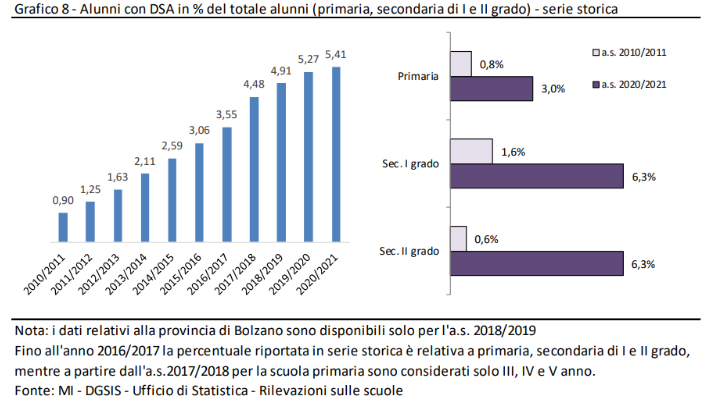
\includegraphics[width=0.9\textwidth]{img/statistica_italia.png}
\par
In particolare, nel 2020/2021, si contavano un totale di 326.548 \textsuperscript{\cite{miur}} di cui:
\begin{itemize} 
    \item \textbf{48.022 studenti} con DSA nella scuola primaria.
    \item \textbf{107.389 studenti} con DSA nella scuola secondaria di primo grado.
    \item \textbf{171.137 studenti }con DSA nella scuola secondaria di secondo grado
\end{itemize}
\noindent
\textbf{A cosa è dovuto questo aumento?}
\par
Sicuramente l’applicazione della legge 170/2010 ha giocato un ruolo fondamentale in questo aumento. Le tecniche diagnostiche e la formazione di psicologici e neurologici sono migliorate in questi anni e ciò permette di riconoscere e intervenire sui DSA già a partire dalla scuola primaria. Inoltre i cambiamenti nei contesti sociali e familiari e un'attenzione maggiore verso il benessere psicologico hanno motivato le famiglie ad una maggiore attenzione verso eventuali difficoltà scolastiche dei figli, aumentando i casi riconosciuti.
\par
Negli Stati Uniti i disturbi specifici dell'apprendimento sono regolamenti all'interno dell'IDEA (“Individuals with Disabilities Education Act”), fonte normativa che considera i DSA all’interno delle disabilità . L’IDEA, attraverso programmi specifici (“Individualized Education Program, IEP”), garantisce un'istruzione pubblica gratuita, appropriata e personalizzata.
\par
Nel 2021/2022, da una ricerca National Center for Education Statistics (NCES), il numero di studenti che hanno usufruito dell’IDEA è stato di circa 7,3 milioni, equivalente al 15\% di tutti gli studenti delle scuole pubbliche, tra un'età compresa tra i 3 e 21 anni. In particolare la categoria maggiormente rappresentativa erano i DSA con il 32\% \textsuperscript{\cite{nces}}.
\par
Una principale differenza tra le due legislazioni riguarda la considerazione negli USA dei DSA come disabilità, mentre la legge italiana considera i DSA come una categoria distinta. La legge 170/2010 evita di equiparare i DSA alle disabilità fisiche o cognitive, evidenziando piuttosto che si tratta di una forma di difficoltà specifica nell’apprendimento.
\par
Le risorse tecnologiche utili all’apprendimento in entrambe le norme non sono definite, lasciando spazio di valutazione ai singoli istituti o ai singoli stati considerando le difficoltà dei DSA e nel caso americano di tutti gli studenti con disabilità.
\par
L’utilizzo di nuove strumentazioni tecnologiche, ad esempio le lavagne LIM (Lavagne interattive multimediali) e tablet a supporto dell’insegnamento, hanno permesso lo sviluppo di software di video-scrittura e lo sviluppo di applicazioni utili all’apprendimento, tra cui l’app SimpleMind Pro utilizzata come base per la creazione di mappe concettuali per questo nostro progetto. Nei successivi paragrafi spiegheremo la creazione delle Mappe concettuali attraverso LaTex, strumento utile per la didattica.

%--------------- \nuova pagina ---------------
\newpage
\newgeometry{top=2cm, bottom=2cm, left=2cm, right=2cm}

\section{Il progetto}  
L’approccio adottato per la traduzione delle mappe concettuali in linguaggio LaTex ha richiesto un’attenta considerazione di diversi fattori per raggiungere l’obiettivo principale di mantenere una fedeltà alle idee originali assicurando al contempo che risultano efficaci e accessibili.
\par
Le mappe concettuali sono state realizzate utilizzando LaTex e la libreria TikZ\textsuperscript{\cite{Tikz}}, nota per l’abilità di creare diagrammi complessi in modo preciso e personalizzabile permettendo di mantenere la struttura gerarchica e le connessioni logiche delle mappe concettuali. La struttura \'{e} stata organizzata a partire da un nodo centrale da quale partono nodi secondari che rappresentano i temi principali. Ogni nodo secondario a sua volta può includere ulteriori nodi figli, che approfondiscono i contenuti tematici in dettaglio.
\par
Dopo l’installazione e il setup del pacchetto TikZ si può proseguire alla creazione, di seguito sono mostrati alcuni modi in cui lo abbiamo utilizzato:
\begin{itemize} 
    \item Creazione dei nodi, che rappresentano i concetti principali e adiacenti di un argomento:
        \begin{quote}
            \textit{\textbackslash node[concept color=blue!60] {Concetto Principale};}
        \end{quote}
    \item Connessioni tra nodi rappresentano le relazioni logiche tra i concetti. TikZ ci permette di disegnare linee o frecce, personalizzabili in termine di direzione e stile, tra i nodi per indicare queste relazioni;
    \item Struttura gerarchica:
        \begin{quote}
            \textit{\textbackslash node[concept] {Concetto Generale}\\
               	    \textbackslash child { \textbackslash node[concept] {Concetto Specifico 1} }\\
                        \textbackslash child { \textbackslash node[concept] {Concetto Specifico 2} };}
        \end{quote}
\end{itemize}
Durante il processo di creazione delle mappe, sono state adottate anche specifiche strategie per ottimizzare la rappresentazione grafica e la leggibilità come la regolazione degli angoli tra i nodi figli, la personalizzazione delle distanze e l’uso di colori diversi per differenziare i vari livelli. In questo modo si \'{e} evitata la sovrapposizione tra le bolle, migliorando la distribuzione spaziale e l’estetica complessiva. 
\par
Di seguito sono riportati dettagli tecnici che si sono utilizzati per la ottimizzazione visiva:
\begin{itemize} 
    \item L’organizzazione degli angoli e delle distanze dei nodi figli:
        \begin{itemize}
            \item Sono stati personalizzati gli angoli di separazione tra i nodi figli, per evitare la sovrapposizione dei nodi e dei testi adiacenti con l’uso del parametro sibling angle;
            \item È stata modificata la lunghezza dei collegamenti tra i nodi tramite level distance per garantire una separazione chiara tra le bolle.
        \end{itemize}
    \item La personalizzazione dei colori:
        \begin{itemize}
            \item I colori dei nodi sono stati modificati utilizzando le tonalità fornite dalla libreria xcolor. Ogni nodo ha un colore distinto per migliorare la leggibilità e migliorare l’identificazione tematica, come yellow!40 che indica una combinazione di 40\% di giallo e 60\% bianco.
        \end{itemize}
    \item La gestione del testo nei nodi:
        \begin{itemize}
            \item Il testo dei nodi può essere modificato in modo da accogliere il testo meglio, con l’aiuto di textwidth=10em. Così si garantisce la leggibilità del testo.
        \end{itemize}
\end{itemize}
L'uso di questo pacchetto ha permesso di evitare un'eccessiva complessità tecnica, concentrandosi invece su come la tecnologia possa supportare l'apprendimento inclusivo. La possibilità di personalizzare colori, forme e connessioni ha reso le mappe concettuali più accessibili, facilitando la comprensione e l'interazione con il materiale didattico.
\par
In questo modo, la tecnologia si è dimostrata un alleato potente nel rendere l'apprendimento più personalizzato, rispondendo alle diverse esigenze degli studenti con DSA. 
Nella parte successiva, verrà illustrata la parte tecnica di LaTex trattata dal nostro gruppo, illustrando come queste personalizzazioni possano essere implementate per migliorare ulteriormente l'efficacia didattica.

\subsection{Elenco delle funzioni utilizzate} 
Il progetto è costituito da diverse cartelle, contenenti files suddivisi per utilizzo.
\par
All’interno della cartella \textbf{config} ci sono i seguenti files:
\begin{itemize}
    \item \textbf{packages-imports.tex}: è un insieme di comandi in LaTeX che configura l'aspetto del documento, aggiungendo funzionalità per personalizzare intestazioni e piè di pagina, creare elenchi, disegnare figure e impostare caratteri specifici;
    \item \textbf{custom-commands.tex}: è un insieme di comandi in LaTeX che configura vari elementi di formattazione e layout, tra cui intestazioni personalizzate, regole orizzontali, liste numerate e box informativi; 
    \item \textbf{document-header.tex}: Il codice LaTeX descritto in questo file configura l’intestazione del documento, allineando il logo e le informazioni istituzionali, separando visivamente le sezioni con linee e spazi, e centrando il nome del progetto e il link al repository per una chiara visualizzazione delle informazioni iniziali;
    \item \textbf{hyperef.doc.info.tex}: Il codice LaTeX viene utilizzato per configurare i metadati nel documento PDF generato dal compilatore LaTeX. I metadati sono informazioni aggiuntive che vengono incorporati nel PDF e che non sono visibili nel corpo del documento, ma che possono essere lette da software di visualizzazione PDF o da strumenti di ricerca.
\end{itemize}
\par
All’interno della cartella \textbf{data} sono contenuti file contenenti informazioni su dati da inserire all’interno del documento, come: autori del progetto, materia di studio, ecc; ma anche schemi e mappe concettuali che essendo esterne al documento principale sonno essere spostate facilmente in posto diverso all’interno del documento.
\par
All’interno della cartella \textbf{img} sono inserite tutte le immagini utilizzate all’interno del progetto.
\par
Il file principale, \textbf{MappeConcettuali.tex}, è nella root del progetto e contiene i richiami ai file descritti sopra, oltre a tutto il progetto.\\
\par
\noindent
Pacchetti base utilizzati:
\begin{itemize}
    \item \textbf{\textbackslash usepackage\{fancyhdr, lastpage, bbding, pmboxdraw\}}:
        \begin{itemize}
            \item \textbf{fancyhdr}: permette di personalizzare le intestazioni e i piè di pagina del documento. Fornisce comandi per modificare il contenuto di questi elementi;
            \item \textbf{lastpage}: consente di riferirsi all'ultima pagina del documento, utile per numerare le pagine in formati tipo "Pagina X di Y";
            \item \textbf{bbding}: include un insieme di simboli decorativi e segni di spunta che possono essere usati per creare elenchi o evidenziare parti del testo;
            \item \textbf{pmboxdraw}: include una serie di simboli utili per disegnare bordi e riquadri di testo.
        \end{itemize}
    \item \textbf{\textbackslash usepackage\{titlesec\}}: permette di personalizzare l’aspetto dei titoli di sezioni e sottosezioni, regolando font, dimensioni e spaziatura.
    \item \textbf{\textbackslash usepackage\{fontspec\}}: fontspec è un pacchetto che consente di usare caratteri specifici con XeLaTeX o LuaLaTeX. In questo caso è stato scelto il carattere OpenDyslexic\footnote{ (https://opendyslexic.org/)}, che può migliorare la leggibilità per persone con dislessia. Il comando \setmainfont{OpenDyslexic} imposta il carattere OpenDyslexic come font principale del documento.
    \item \textbf{\textbackslash usepackage\{tikz\}}: TikZ è un pacchetto per creare grafici e diagrammi direttamente in LaTeX.
\end{itemize}
\par
\noindent
Librerie base utilizzate:
\begin{itemize}
    \item \textbf{\textbackslash usetikzlibrary\{mindmap, shadows, trees, positioning\}}. Di seguito alcuni delle opzioni utilizzate:
        \begin{itemize}
            \item \textbf{mindmap}: permette di creare mappe mentali;
            \item \textbf{shadows}: aggiunge ombre agli elementi grafici per dare un effetto tridimensionale;
            \item \textbf{trees}: fornisce strumenti per creare strutture ad albero, come grafici gerarchici o alberi genealogici;
            \item \textbf{positioning}: aiuta a posizionare gli elementi di TikZ in modo più preciso;
            \item \textbf{grow cyclic}: specifica che i nodi figli (o rami) saranno disposti in un cerchio attorno al nodo genitore. Ogni nodo figlio è posizionato a intervalli angolari uguali (o specificati manualmente) rispetto al centro;
        \end{itemize}
\end{itemize}
\par
\noindent
Principali comandi utilizzati:
\begin{itemize}
    \item \textbf{\textbackslash node{}}: Serve per creare un elemento grafico (un nodo) in un diagramma. Un nodo è un punto di ancoraggio che può contenere testo, simboli o grafica e che può essere collegato ad altri nodi tramite linee, frecce o curve.\\
    \textbf{Sintassi:}\textbackslash node[opzioni](nome\_coordinata)\{contenuto\};\\
    \textbf{Componenti principali}
        \begin{itemize}
            \item \textbf{[opzioni]} (facoltativo): permette di configurare l'aspetto del nodo (ad esempio, colore, forma, posizione);
            \item \textbf{(nome\_coordinata)} (facoltativo): identifica il nodo con un nome, utile per riferimenti successivi (ad esempio, per disegnare frecce verso questo nodo);
            \item \textbf{\{contenuto\}} (obbligatorio): contiene il testo o l'elemento grafico da visualizzare all'interno del nodo.
        \end{itemize}
     \item \textbf{\textbackslash child{}}: Serve per creare nodi figli in una struttura gerarchica (come una mappa concettuale o un albero). Ogni nodo creato con \textbackslash child diventa un figlio del nodo genitore, che si trova al livello immediatamente superiore nella gerarchia.\\
     \textbf{Sintassi:}\textbackslash child{ node[opzioni] \{contenuto\} };\\
     \textbf{Componenti principali}:
     \begin{itemize}
            \item \textbf{node[opzioni]}: specifica lo stile del nodo figlio, ad esempio la forma, il colore, o il contenuto;
            \item \textbf{\{contenuto}\}: contiene il testo o la grafica del nodo figlio;
    \end{itemize}
    \item \textbf{\textbackslash draw{}}: è utilizzato per disegnare linee, curve, forme e altre strutture grafiche.\\
    \textbf{Sintassi:}\textbackslash draw[opzioni] (punto1) -- (punto2) -- ... -- (puntoN);\\
    \textbf{Componenti principali}:
        \begin{itemize}
            \item \textbf{[opzioni]} (facoltativo): specifica lo stile del disegno, come colore, spessore, tratteggio, ecc.;
            \item \textbf{(punto1), (punto2), ...}: specifica i punti del percorso da disegnare. I punti possono essere specificati come coordinate assolute (x, y) o relative ++(dx, dy).
        \end{itemize}
    \item \textbf{\textbackslash path\{\}}: è utilizzato per definire un percorso senza disegnarlo visivamente. È simile al comando \textbackslash draw, ma non produce alcuna grafica visibile di default. È particolarmente utile per definire percorsi, posizionare nodi o calcolare coordinate, lasciando la possibilità di aggiungere elementi grafici separatamente.\\
    \textbf{Sintassi:}\textbackslash path[opzioni] (punto1) -- (punto2) -- ... -- (puntoN);\\
    \textbf{Componenti principali}:
        \begin{itemize}
            \item \textbf{[opzioni]} (facoltativo): definisce le caratteristiche del percorso (simile a \textbackslash draw), come stile e comportamento;
            \item \textbf{(punto1), (punto2), ...}: specifica i punti del percorso da disegnare. I punti possono essere specificati come coordinate assolute (x, y) o relative ++(dx, dy).
        \end{itemize}
\end{itemize}

%--------------- \nuova pagina ---------------
\newpage
\newgeometry{top=2cm, bottom=2cm, left=2cm, right=2cm}

\section{Mappa "Il software"}

%--------------- Importa il workflow di git --------------- 
\flushleft
\resizebox{7.2in}{!}{
    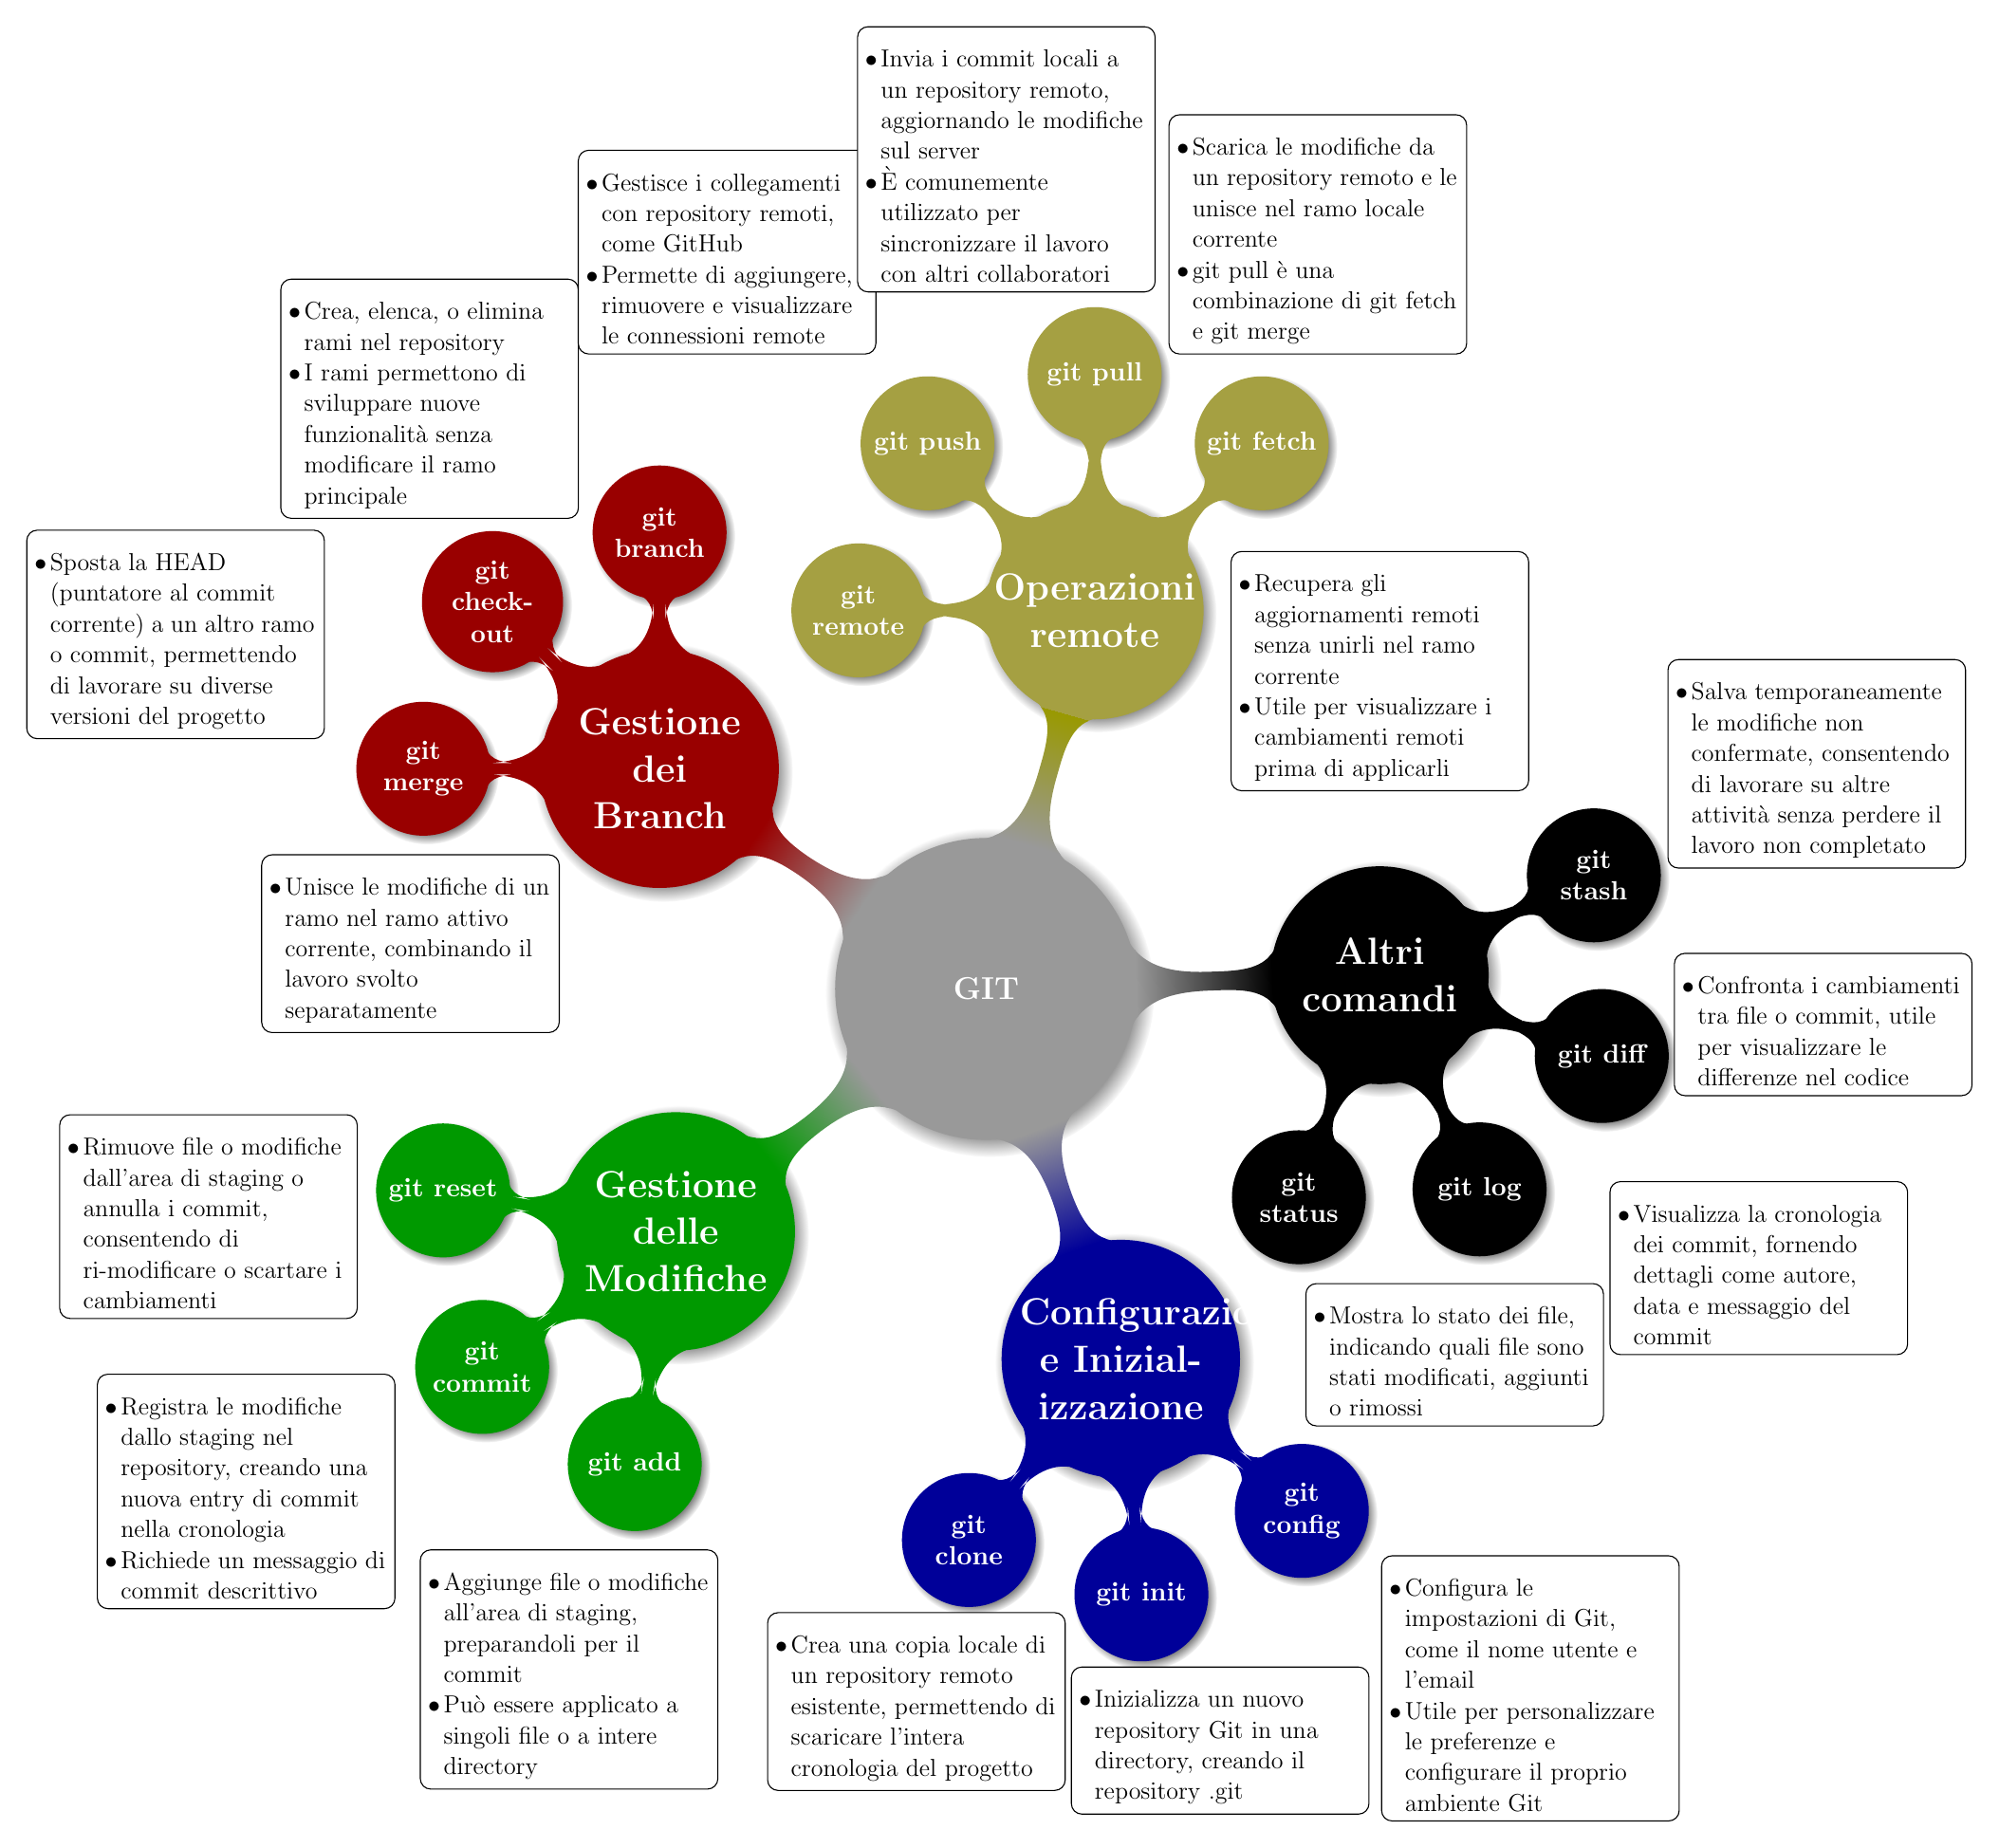
\begin{tikzpicture}[ every annotation/.style = {draw,
                     fill = white, font = \Large}]
  \path[mindmap,concept color=black!40,text=white,
    every node/.style={concept,circular drop shadow},
    git/.style    = {concept color=black!40,font=\large\bfseries,text width=10em},
    level 1 concept/.append style={font=\Large\bfseries,sibling angle=72,text width=7.7em,level distance=15em,inner sep=0pt},
    level 2 concept/.append style={font=\bfseries,sibling angle=45,level distance=9em}]
    
  node[git] {GIT} [clockwise from=290]
    child[concept color=blue!60!black] {
      node[concept] (c_i) {Configurazione e Inizializzazione}[clockwise from=320]
      child { node[concept] (config) {git config} }
      child { node[concept] (init) {git init} }
      child { node[concept] (clone) {git clone}}
    }
    child[concept color=green!60!black] {
      node[concept] (g_m) {Gestione delle Modifiche}[clockwise from=260]
      child { node[concept] (add) {git add} }
      child { node[concept] (commit) {git commit} }
      child { node[concept] (reset) {git reset} }
    }
    child[concept color=red!60!black] {
      node[concept] (g_b) {Gestione dei Branch}[counterclockwise from=90]
      child { node[concept] (branch) {git branch}}
      child { node[concept] (checkout) {git checkout} }
      child { node[concept] (merge) {git merge} }
    }
    child[concept color=yellow!60!black] {
      node[concept] (o_r) {Operazioni remote} [clockwise from=180]
      child { node[concept] (remote) {git remote}}
      child { node[concept] (push) {git push} }
      child { node[concept] (pull) {git pull} }
      child { node[concept] (fetch) {git fetch} }
    }
    child[concept color=black!60!black] {
      node[concept] (a_c) {Altri comandi} [counterclockwise from=250]
      child { node[concept] (status) {git status}}
      child { node[concept] (log) {git log} }
      child { node[concept] (diff) {git diff} }
      child { node[concept] (stash) {git stash} }
    };
    
    \info{config.south east}{right,anchor=west,xshift=1em,yshift=-5em}{%
      \item Configura le impostazioni di Git, come il nome utente e l'email
      \item Utile per personalizzare le preferenze e configurare il proprio ambiente Git
    }
    \info{init.south}{below,anchor=north,xshift=3em,yshift=0em}{%
      \item Inizializza un nuovo repository Git in una directory, creando il repository .git
    }
    \info{clone.south}{below,anchor=north,xshift=-2em,yshift=0em}{%
      \item Crea una copia locale di un repository remoto esistente, permettendo di scaricare l'intera cronologia del progetto
    }
    \info{add.south}{left,anchor=north,xshift=-2.5em,yshift=-0.5em}{%
      \item Aggiunge file o modifiche all'area di staging, preparandoli per il commit
      \item Può essere applicato a singoli file o a intere directory
    }
    \info{commit.west}{left,anchor=north,xshift=-6.5em,yshift=0em}{%
      \item Registra le modifiche dallo staging nel repository, creando una nuova entry di commit nella cronologia
      \item Richiede un messaggio di commit descrittivo
    }
    \info{reset.west}{left,anchor=east,xshift=-0.5em,yshift=-1em}{%
      \item Rimuove file o modifiche dall'area di staging o annulla i commit, consentendo di ri-modificare o scartare i cambiamenti
    }
    \info{branch.north west}{left,anchor=south,xshift=-7em,yshift=-1.5em}{%
      \item Crea, elenca, o elimina rami nel repository
      \item I rami permettono di sviluppare nuove funzionalità senza modificare il ramo principale
    }
    \info{checkout.west}{right,anchor=north east,xshift=-3.5em,yshift=3em}{%
      \item Sposta la HEAD (puntatore al commit corrente) a un altro ramo o commit, permettendo di lavorare su diverse versioni del progetto
    }
    \info{merge.west}{right,anchor=north,xshift=2em,yshift=-3em}{%
      \item Unisce le modifiche di un ramo nel ramo attivo corrente, combinando il lavoro svolto separatamente
    }
    \info{remote.north}{above,anchor=south,xshift=-5em,yshift=7em}{%
      \item Gestisce i collegamenti con repository remoti, come GitHub
      \item Permette di aggiungere, rimuovere e visualizzare le connessioni remote
    }
    \info{push.north}{above,anchor=south,xshift=3em,yshift=3em}{%
      \item Invia i commit locali a un repository remoto, aggiornando le modifiche sul server
      \item È comunemente utilizzato per sincronizzare il lavoro con altri collaboratori
    }
    \info{pull.north}{above,anchor=south,xshift=8.5em,yshift=-2em}{%
      \item Scarica le modifiche da un repository remoto e le unisce nel ramo locale corrente
      \item git pull è una combinazione di git fetch e git merge
    }
    \info{fetch.north}{above,anchor=south,xshift=4.5em,yshift=-16em}{%
      \item Recupera gli aggiornamenti remoti senza unirli nel ramo corrente
      \item Utile per visualizzare i cambiamenti remoti prima di applicarli
    }
    \info{status.east}{left,anchor=west,xshift=-2.5em,yshift=-6em}{%
      \item Mostra lo stato dei file, indicando quali file sono stati modificati, aggiunti o rimossi
    }
    \info{log.east}{left,anchor=west,xshift=2.2em,yshift=-3em}{%
      \item Visualizza la cronologia dei commit, fornendo dettagli come autore, data e messaggio del commit
    }
    \info{diff.east}{left,anchor=west,xshift=0em,yshift=1.2em}{%
      \item Confronta i cambiamenti tra file o commit, utile per visualizzare le differenze nel codice
    }
    \info{stash.east}{left,anchor=south,xshift=6em,yshift=0em}{%
      \item Salva temporaneamente le modifiche non confermate, consentendo di lavorare su altre attività senza perdere il lavoro non completato
    }
;
\end{tikzpicture}
}

%--------------- \nuova pagina ---------------
\newpage
\newgeometry{top=2cm, bottom=2cm, left=2cm, right=2cm}

\section{Mappa "GIT workflow"} 

%--------------- Importa il workflow di git --------------- 
\flushleft
\resizebox{7.2in}{!}{
    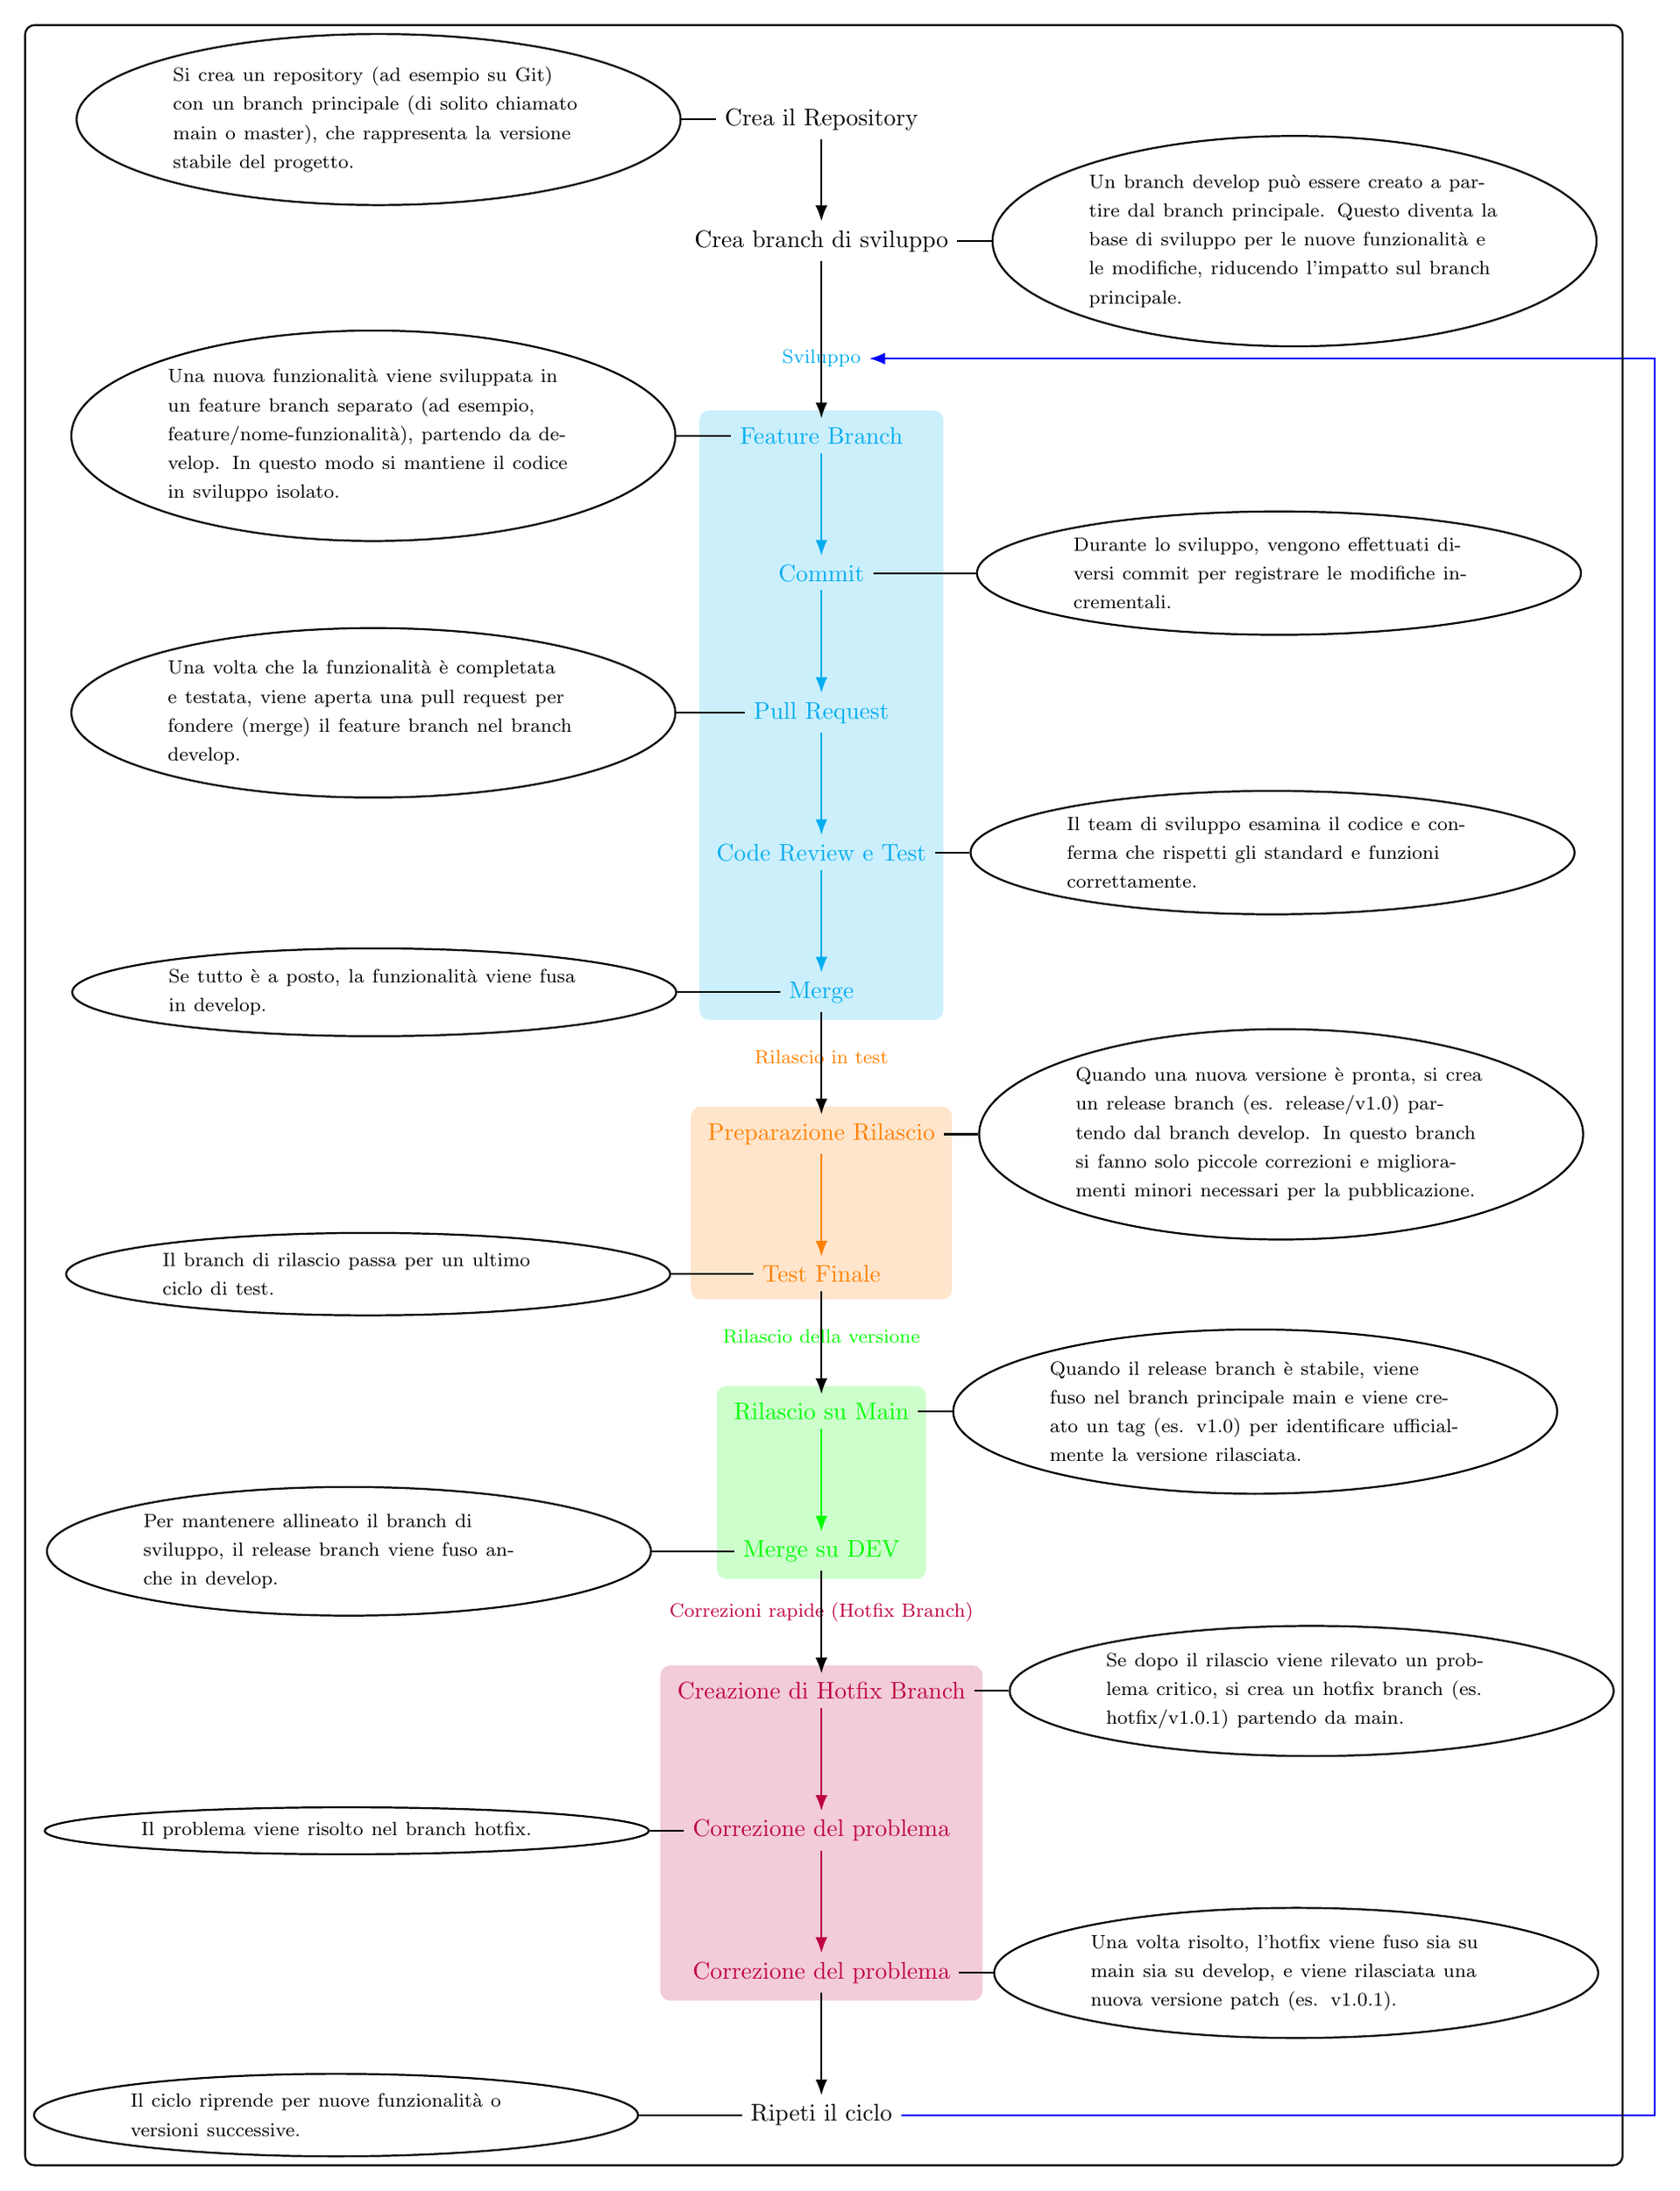
\begin{tikzpicture}[>=Latex,thick]
        
    % Nodo principale per la creazione del repository
        \node (REPO) {Crea il Repository};
        % Aggiunta di una descrizione per REPO
        \node[ellipse,draw, left=0.5cm of REPO, text width=6cm, align=left] (REPO_DESC) {\footnotesize Si crea un repository (ad esempio su Git) con un branch principale (di solito chiamato main o master), che rappresenta la versione stabile del progetto.};
        
    % Nodo per la creazione del branch di sviluppo
        \node[below=1.2cm of REPO] (B_DEV) {Crea branch di sviluppo};
        % Aggiunta di una descrizione per B_DEV
        \node[ellipse,draw, right=0.5cm of B_DEV, text width=6cm, align=left] (B_DEV_DESC) {\footnotesize Un branch develop può essere creato a partire dal branch principale. Questo diventa la base di sviluppo per le nuove funzionalità e le modifiche, riducendo l'impatto sul branch principale.};
        
    % Nodo Feature Branche
        \node[below=2.3cm of B_DEV, cyan] (FB) {Feature Branch}; 
        % Aggiunta di una descrizione per FB
        \node[ellipse,draw, left=0.8cm of FB, text width=6cm, align=left] (FB_DESC) {\footnotesize Una nuova funzionalità viene sviluppata in un feature branch separato (ad esempio, feature/nome-funzionalità), partendo da develop. In questo modo si mantiene il codice in sviluppo isolato.};

    %Nodo Commit
        \node[below=1.5cm of FB, cyan] (COMMIT) {Commit};
        % Aggiunta di una descrizione per COMMIT
        \node[ellipse,draw, right=1.5cm of COMMIT, text width=6cm, align=left] (COMMIT_DESC) {\footnotesize Durante lo sviluppo, vengono effettuati diversi commit per registrare le modifiche incrementali.};

    %Nodo Pull Request
        \node[below=1.5cm of COMMIT, cyan] (PR) {Pull Request};
        % Aggiunta di una descrizione per Pull Request
        \node[ellipse,draw, left=1cm of PR, text width=6cm, align=left] (PR_DESC) {\footnotesize Una volta che la funzionalità è completata e testata, viene aperta una pull request per fondere (merge) il feature branch nel branch develop.};

    %Nodo Code Review e Test
        \node[below=1.5cm of PR, cyan] (CRT) {Code Review e Test};
        % Aggiunta di una descrizione per Code Review e Test
        \node[ellipse,draw, right=0.5cm of CRT, text width=6cm, align=left] (CRT_DESC) {\footnotesize Il team di sviluppo esamina il codice e conferma che rispetti gli standard e funzioni correttamente.};     

    %Nodo Merge
        \node[below=1.5cm of CRT, cyan] (MRG) {Merge};
        % Aggiunta di una descrizione per Merge
        \node[ellipse,draw, left=1.5cm of MRG, text width=6cm, align=left] (MRG_DESC) {\footnotesize Se tutto è a posto, la funzionalità viene fusa in develop.};


    % Creazione del rettangolo (Sviluppo)
        \begin{scope}[on background layer]
            \node[fit=(FB)(COMMIT)(PR)(CRT)(MRG),fill=cyan!20,rounded corners] (RCTL_1) {};
            \node[above=0.5cm of RCTL_1,cyan](SV){\footnotesize Sviluppo};
        \end{scope}

    %Nodo Preparazione Rilascio
        \node[below=1.5cm of MRG, orange] (P_RIL) {Preparazione Rilascio};
        % Aggiunta di una descrizione per Preparazione Rilascio
        \node[ellipse,draw, right=0.5cm of P_RIL, text width=6cm, align=left] (P_RIL_DESC) {\footnotesize Quando una nuova versione è pronta, si crea un release branch (es. release/v1.0) partendo dal branch develop. In questo branch si fanno solo piccole correzioni e miglioramenti minori necessari per la pubblicazione.};

    %Nodo Test Finale
        \node[below=1.5cm of P_RIL, orange] (TF) {Test Finale};
        % Aggiunta di una descrizione per Test Finale
        \node[ellipse,draw, left=1.2cm of TF, text width=6cm, align=left] (TF_DESC) {\footnotesize Il branch di rilascio passa per un ultimo ciclo di test.};

    % Creazione del rettangolo (rilascio in test)
        \begin{scope}[on background layer]
            \node[fit=(P_RIL)(TF),fill=orange!20,rounded corners] (RCTL_2) {};
            \node[above=0.5cm of RCTL_2,orange](RT){\footnotesize Rilascio in test};
        \end{scope}

    %Nodo Merge su Main
        \node[below=1.5cm of TF, green] (RIL) {Rilascio su Main};
        % Aggiunta di una descrizione per Preparazione Rilascio
        \node[ellipse,draw, right=0.5cm of RIL, text width=6cm, align=left] (RIL_DESC) {\footnotesize Quando il release branch è stabile, viene fuso nel branch principale main e viene creato un tag (es. v1.0) per identificare ufficialmente la versione rilasciata.};

    %Nodo Merge su Develop
        \node[below=1.5cm of RIL, green] (RIL_DEV) {Merge su DEV};
        % Aggiunta di una descrizione per Test Finale
        \node[ellipse,draw, left=1.2cm of RIL_DEV, text width=6cm, align=left] (RIL_DEV_DESC) {\footnotesize Per mantenere allineato il branch di sviluppo, il release branch viene fuso anche in develop.};

    % Creazione del rettangolo (rilascio in test)
        \begin{scope}[on background layer]
            \node[fit=(RIL)(RIL_DEV),fill=green!20,rounded corners] (RCTL_3) {};
            \node[above=0.5cm of RCTL_3,green](RT){\footnotesize Rilascio della versione};
        \end{scope}

    %Nodo Creazione di Hotfix Branch
        \node[below=1.5cm of RIL_DEV, purple] (HOT_B) {Creazione di Hotfix Branch};
        % Aggiunta di una descrizione per Preparazione Rilascio
        \node[ellipse,draw, right=0.5cm of HOT_B, text width=6cm, align=left] (HOT_B_DESC) {\footnotesize Se dopo il rilascio viene rilevato un problema critico, si crea un hotfix branch (es. hotfix/v1.0.1) partendo da main.};

    %Nodo Correzione problema
        \node[below=1.5cm of HOT_B, purple] (CORR) {Correzione del problema};
        % Aggiunta di una descrizione per Correzione del problema
        \node[ellipse,draw, left=0.5cm of CORR, text width=6cm, align=left] (CORR_DESC) {\footnotesize Il problema viene risolto nel branch hotfix.};

    %Nodo Correzione problema
        \node[below=1.5cm of CORR, purple] (RIS_HOT_B) {Correzione del problema};
        % Aggiunta di una descrizione per Correzione del problema
        \node[ellipse,draw, right=0.5cm of RIS_HOT_B, text width=6cm, align=left] (RIS_HOT_B_DESC) {\footnotesize Una volta risolto, l’hotfix viene fuso sia su main sia su develop, e viene rilasciata una nuova versione patch (es. v1.0.1).};

    % Creazione del rettangolo (Hotfix Branch)
        \begin{scope}[on background layer]
            \node[fit=(HOT_B)(CORR)(RIS_HOT_B),fill=purple!20,rounded corners] (RCTL_4) {};
            \node[above=0.5cm of RCTL_4,purple](RT){\footnotesize Correzioni rapide (Hotfix Branch)};
        \end{scope}

    %Nodo ripeti ciclo
        \node[below=1.5cm of RIS_HOT_B] (RIP_CICLO) {Ripeti il ciclo};
        % Aggiunta di una descrizione per ripeti ciclo
        \node[ellipse,draw, left=1.5cm of RIP_CICLO, text width=6cm, align=left] (RIP_CICLO_DESC) {\footnotesize Il ciclo riprende per nuove funzionalità o versioni successive.};

        % Creazione delle frecce di connessione
        \draw[->] (REPO) -- (B_DEV);
        \draw[->] (B_DEV) -- (FB);
        \draw[->, cyan] (FB) -- (COMMIT);
        \draw[->, cyan] (COMMIT) -- (PR);
        \draw[->, cyan] (PR) -- (CRT);
        \draw[->, cyan] (CRT) -- (MRG);
        \draw[->] (MRG) -- (P_RIL);
        \draw[->, orange] (P_RIL) -- (TF);
        \draw[->] (TF) -- (RIL);
        \draw[->, green] (RIL) -- (RIL_DEV);
        \draw[->] (RIL_DEV) -- (HOT_B);
        \draw[->, purple] (HOT_B) -- (CORR);
        \draw[->, purple] (CORR) -- (RIS_HOT_B);
        \draw[->] (RIS_HOT_B) -- (RIP_CICLO);

        \draw[->, blue] (RIP_CICLO.east) -- ++(11,0) |- (SV.east);
        
        % Creazione dei trattini di collegamento descrizione
        \draw (REPO) -- (REPO_DESC);
        \draw (B_DEV) -- (B_DEV_DESC);
        \draw (FB) -- (FB_DESC);
        \draw (COMMIT) -- (COMMIT_DESC);
        \draw (PR) -- (PR_DESC);
        \draw (CRT) -- (CRT_DESC);
        \draw (MRG) -- (MRG_DESC);
        \draw (P_RIL) -- (P_RIL_DESC);
        \draw (TF) -- (TF_DESC);
        \draw (RIL) -- (RIL_DESC);
        \draw (RIL_DEV) -- (RIL_DEV_DESC);
        \draw (HOT_B) -- (HOT_B_DESC);
        \draw (CORR) -- (CORR_DESC);
        \draw (RIS_HOT_B) -- (RIS_HOT_B_DESC);
        \draw (RIP_CICLO) -- (RIP_CICLO_DESC);
        
        % Bordo intorno all'intero workflow
        \node[fit=(REPO)(FB_DESC)(REPO_DESC)(B_DEV_DESC)(PR_DESC)(CRT_DESC)(MRG_DESC)(TF_DESC)(P_RIL_DESC)(RIL_DEV_DESC)(RIS_HOT_B_DESC)(RIP_CICLO_DESC)(HOT_B_DESC),rounded corners,draw]{};

    \end{tikzpicture}
    }

%--------------- \nuova pagina ---------------
\newpage
\newgeometry{top=2cm, bottom=2cm, left=2cm, right=2cm}

\section{Mappa "Comandi GIT"} 
%\noindent

%--------------- Importa la mappa dei comandi git --------------- 
\flushleft
\resizebox{7.2in}{!}{
    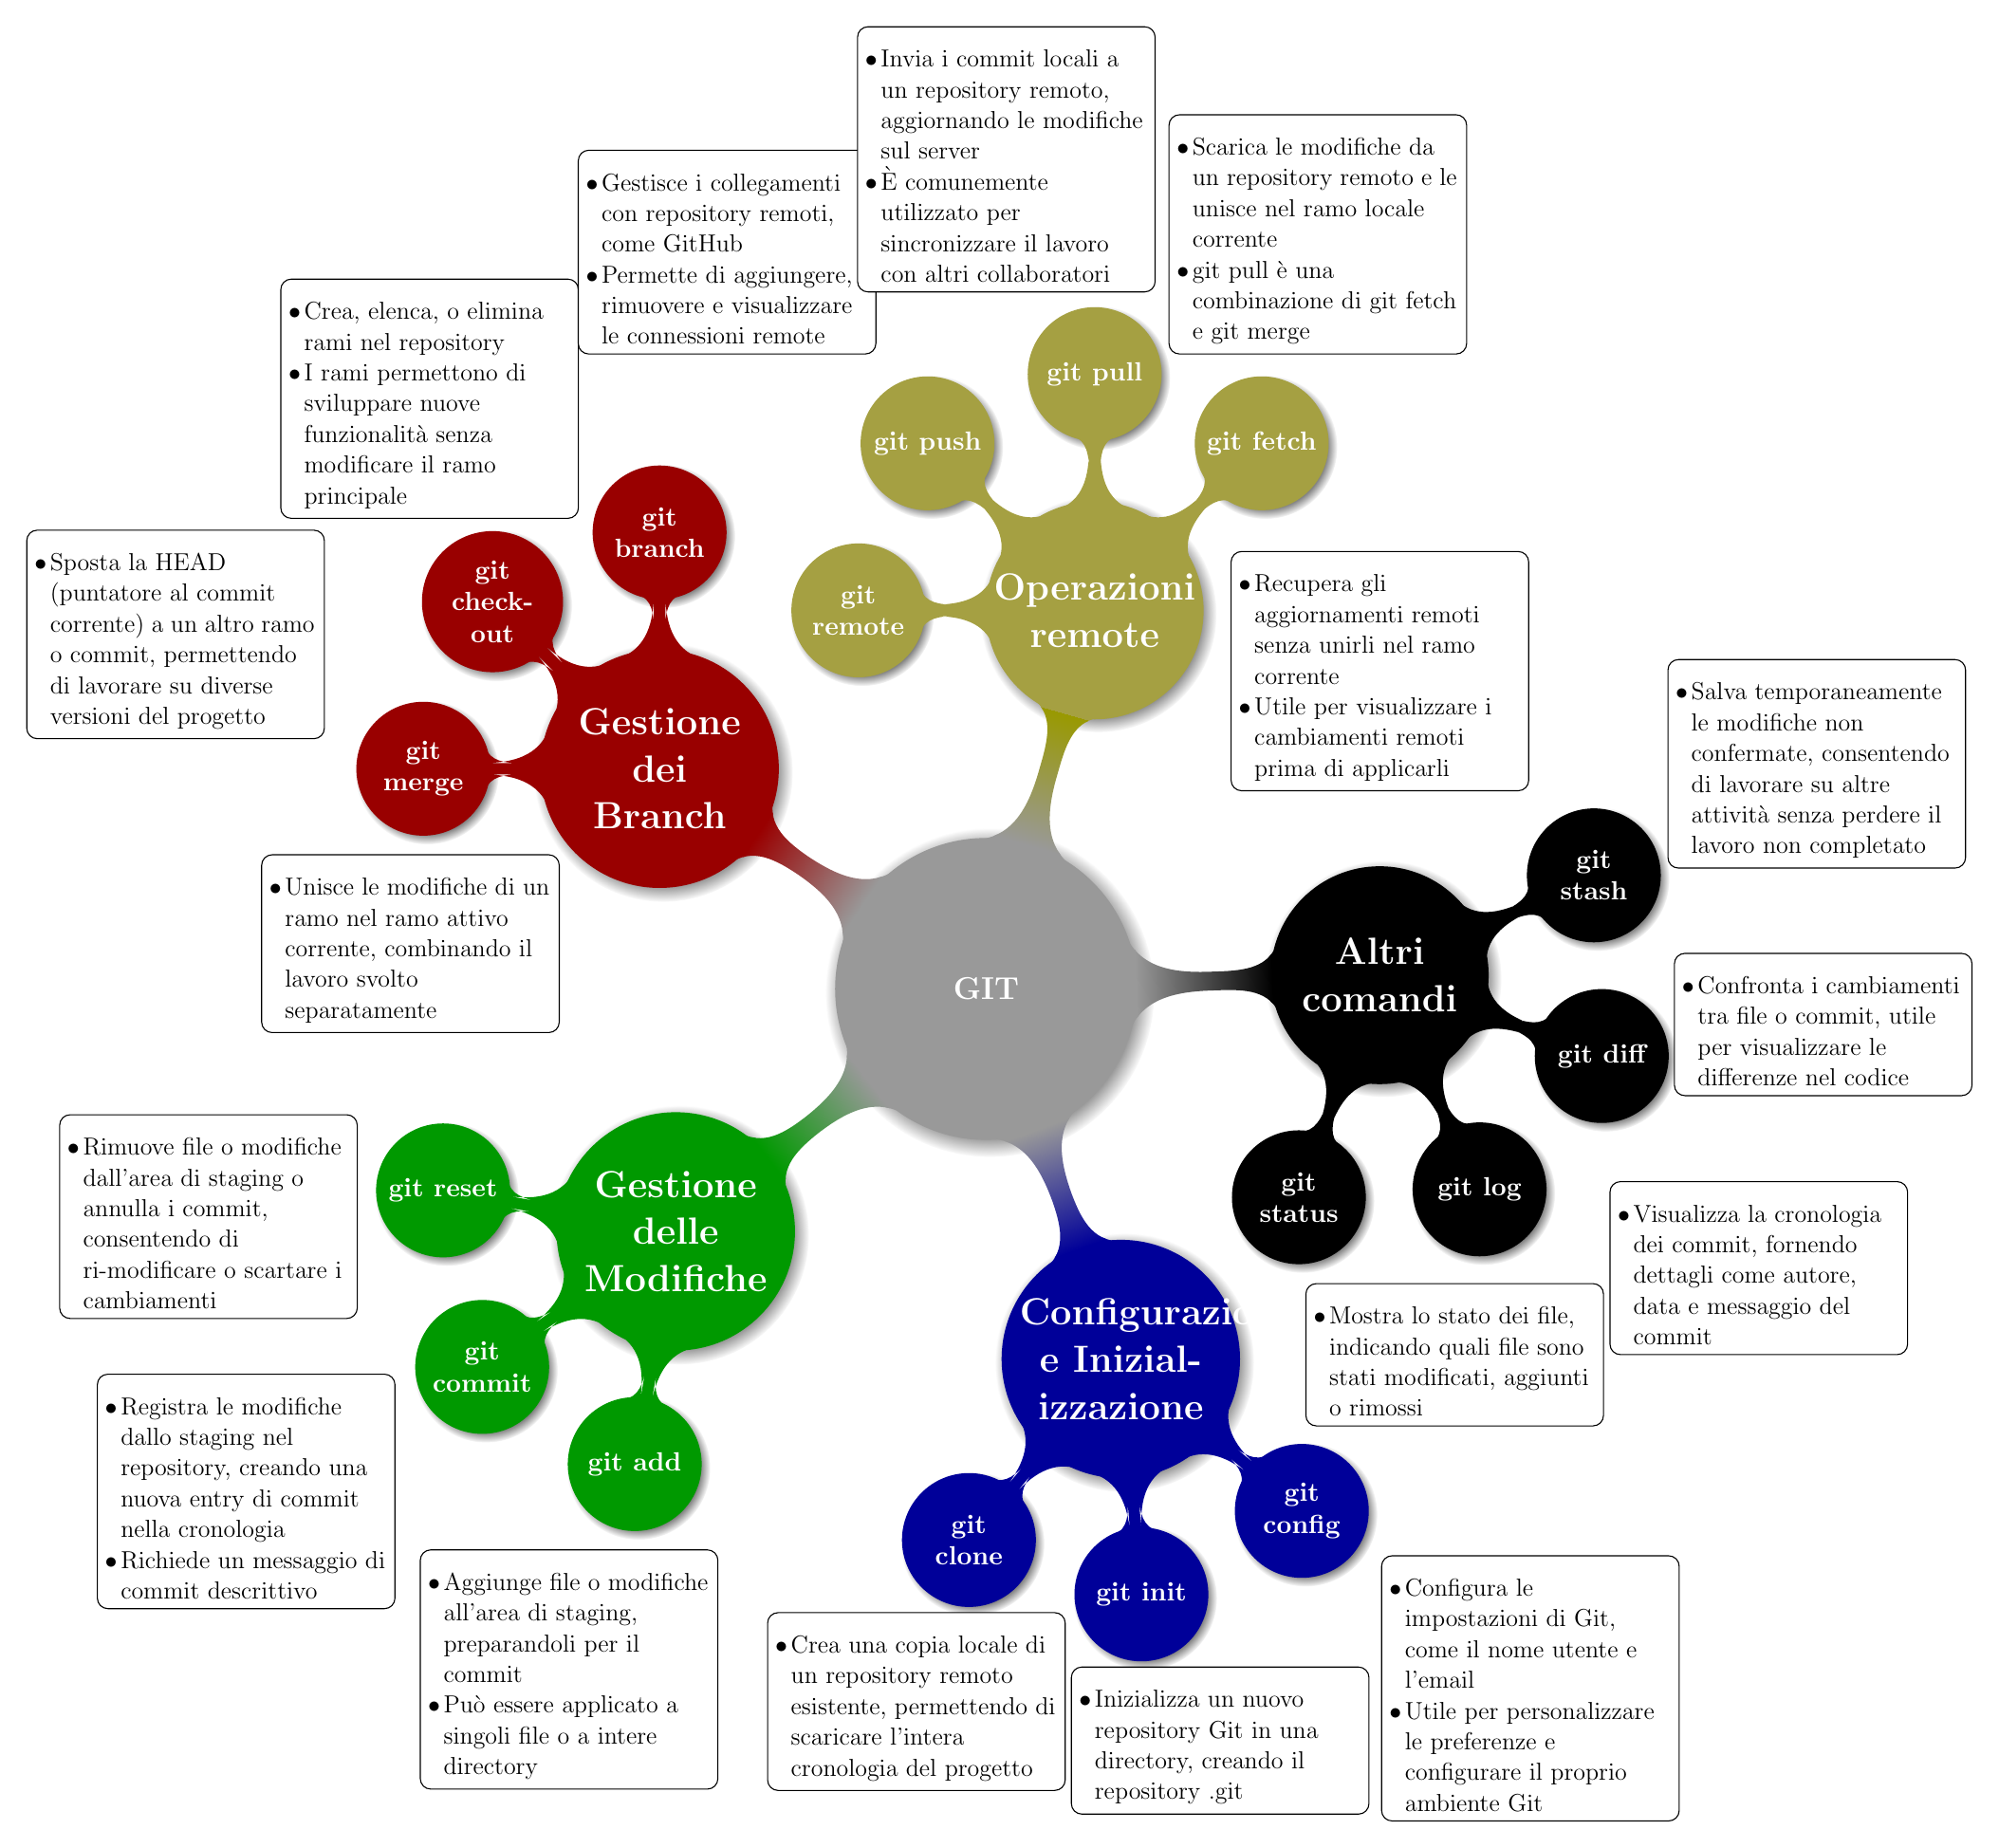
\begin{tikzpicture}[ every annotation/.style = {draw,
                     fill = white, font = \Large}]
  \path[mindmap,concept color=black!40,text=white,
    every node/.style={concept,circular drop shadow},
    git/.style    = {concept color=black!40,font=\large\bfseries,text width=10em},
    level 1 concept/.append style={font=\Large\bfseries,sibling angle=72,text width=7.7em,level distance=15em,inner sep=0pt},
    level 2 concept/.append style={font=\bfseries,sibling angle=45,level distance=9em}]
    
  node[git] {GIT} [clockwise from=290]
    child[concept color=blue!60!black] {
      node[concept] (c_i) {Configurazione e Inizializzazione}[clockwise from=320]
      child { node[concept] (config) {git config} }
      child { node[concept] (init) {git init} }
      child { node[concept] (clone) {git clone}}
    }
    child[concept color=green!60!black] {
      node[concept] (g_m) {Gestione delle Modifiche}[clockwise from=260]
      child { node[concept] (add) {git add} }
      child { node[concept] (commit) {git commit} }
      child { node[concept] (reset) {git reset} }
    }
    child[concept color=red!60!black] {
      node[concept] (g_b) {Gestione dei Branch}[counterclockwise from=90]
      child { node[concept] (branch) {git branch}}
      child { node[concept] (checkout) {git checkout} }
      child { node[concept] (merge) {git merge} }
    }
    child[concept color=yellow!60!black] {
      node[concept] (o_r) {Operazioni remote} [clockwise from=180]
      child { node[concept] (remote) {git remote}}
      child { node[concept] (push) {git push} }
      child { node[concept] (pull) {git pull} }
      child { node[concept] (fetch) {git fetch} }
    }
    child[concept color=black!60!black] {
      node[concept] (a_c) {Altri comandi} [counterclockwise from=250]
      child { node[concept] (status) {git status}}
      child { node[concept] (log) {git log} }
      child { node[concept] (diff) {git diff} }
      child { node[concept] (stash) {git stash} }
    };
    
    \info{config.south east}{right,anchor=west,xshift=1em,yshift=-5em}{%
      \item Configura le impostazioni di Git, come il nome utente e l'email
      \item Utile per personalizzare le preferenze e configurare il proprio ambiente Git
    }
    \info{init.south}{below,anchor=north,xshift=3em,yshift=0em}{%
      \item Inizializza un nuovo repository Git in una directory, creando il repository .git
    }
    \info{clone.south}{below,anchor=north,xshift=-2em,yshift=0em}{%
      \item Crea una copia locale di un repository remoto esistente, permettendo di scaricare l'intera cronologia del progetto
    }
    \info{add.south}{left,anchor=north,xshift=-2.5em,yshift=-0.5em}{%
      \item Aggiunge file o modifiche all'area di staging, preparandoli per il commit
      \item Può essere applicato a singoli file o a intere directory
    }
    \info{commit.west}{left,anchor=north,xshift=-6.5em,yshift=0em}{%
      \item Registra le modifiche dallo staging nel repository, creando una nuova entry di commit nella cronologia
      \item Richiede un messaggio di commit descrittivo
    }
    \info{reset.west}{left,anchor=east,xshift=-0.5em,yshift=-1em}{%
      \item Rimuove file o modifiche dall'area di staging o annulla i commit, consentendo di ri-modificare o scartare i cambiamenti
    }
    \info{branch.north west}{left,anchor=south,xshift=-7em,yshift=-1.5em}{%
      \item Crea, elenca, o elimina rami nel repository
      \item I rami permettono di sviluppare nuove funzionalità senza modificare il ramo principale
    }
    \info{checkout.west}{right,anchor=north east,xshift=-3.5em,yshift=3em}{%
      \item Sposta la HEAD (puntatore al commit corrente) a un altro ramo o commit, permettendo di lavorare su diverse versioni del progetto
    }
    \info{merge.west}{right,anchor=north,xshift=2em,yshift=-3em}{%
      \item Unisce le modifiche di un ramo nel ramo attivo corrente, combinando il lavoro svolto separatamente
    }
    \info{remote.north}{above,anchor=south,xshift=-5em,yshift=7em}{%
      \item Gestisce i collegamenti con repository remoti, come GitHub
      \item Permette di aggiungere, rimuovere e visualizzare le connessioni remote
    }
    \info{push.north}{above,anchor=south,xshift=3em,yshift=3em}{%
      \item Invia i commit locali a un repository remoto, aggiornando le modifiche sul server
      \item È comunemente utilizzato per sincronizzare il lavoro con altri collaboratori
    }
    \info{pull.north}{above,anchor=south,xshift=8.5em,yshift=-2em}{%
      \item Scarica le modifiche da un repository remoto e le unisce nel ramo locale corrente
      \item git pull è una combinazione di git fetch e git merge
    }
    \info{fetch.north}{above,anchor=south,xshift=4.5em,yshift=-16em}{%
      \item Recupera gli aggiornamenti remoti senza unirli nel ramo corrente
      \item Utile per visualizzare i cambiamenti remoti prima di applicarli
    }
    \info{status.east}{left,anchor=west,xshift=-2.5em,yshift=-6em}{%
      \item Mostra lo stato dei file, indicando quali file sono stati modificati, aggiunti o rimossi
    }
    \info{log.east}{left,anchor=west,xshift=2.2em,yshift=-3em}{%
      \item Visualizza la cronologia dei commit, fornendo dettagli come autore, data e messaggio del commit
    }
    \info{diff.east}{left,anchor=west,xshift=0em,yshift=1.2em}{%
      \item Confronta i cambiamenti tra file o commit, utile per visualizzare le differenze nel codice
    }
    \info{stash.east}{left,anchor=south,xshift=6em,yshift=0em}{%
      \item Salva temporaneamente le modifiche non confermate, consentendo di lavorare su altre attività senza perdere il lavoro non completato
    }
;
\end{tikzpicture}
}

%--------------- \nuova pagina ---------------
\newpage
\newgeometry{top=2cm, bottom=2cm, left=2cm, right=2cm}

\section{Mappa "La produzione del software"}  

%--------------- Importa la mappa della produzione del software --------------- 
\flushleft
\resizebox{7.2in}{!}{
    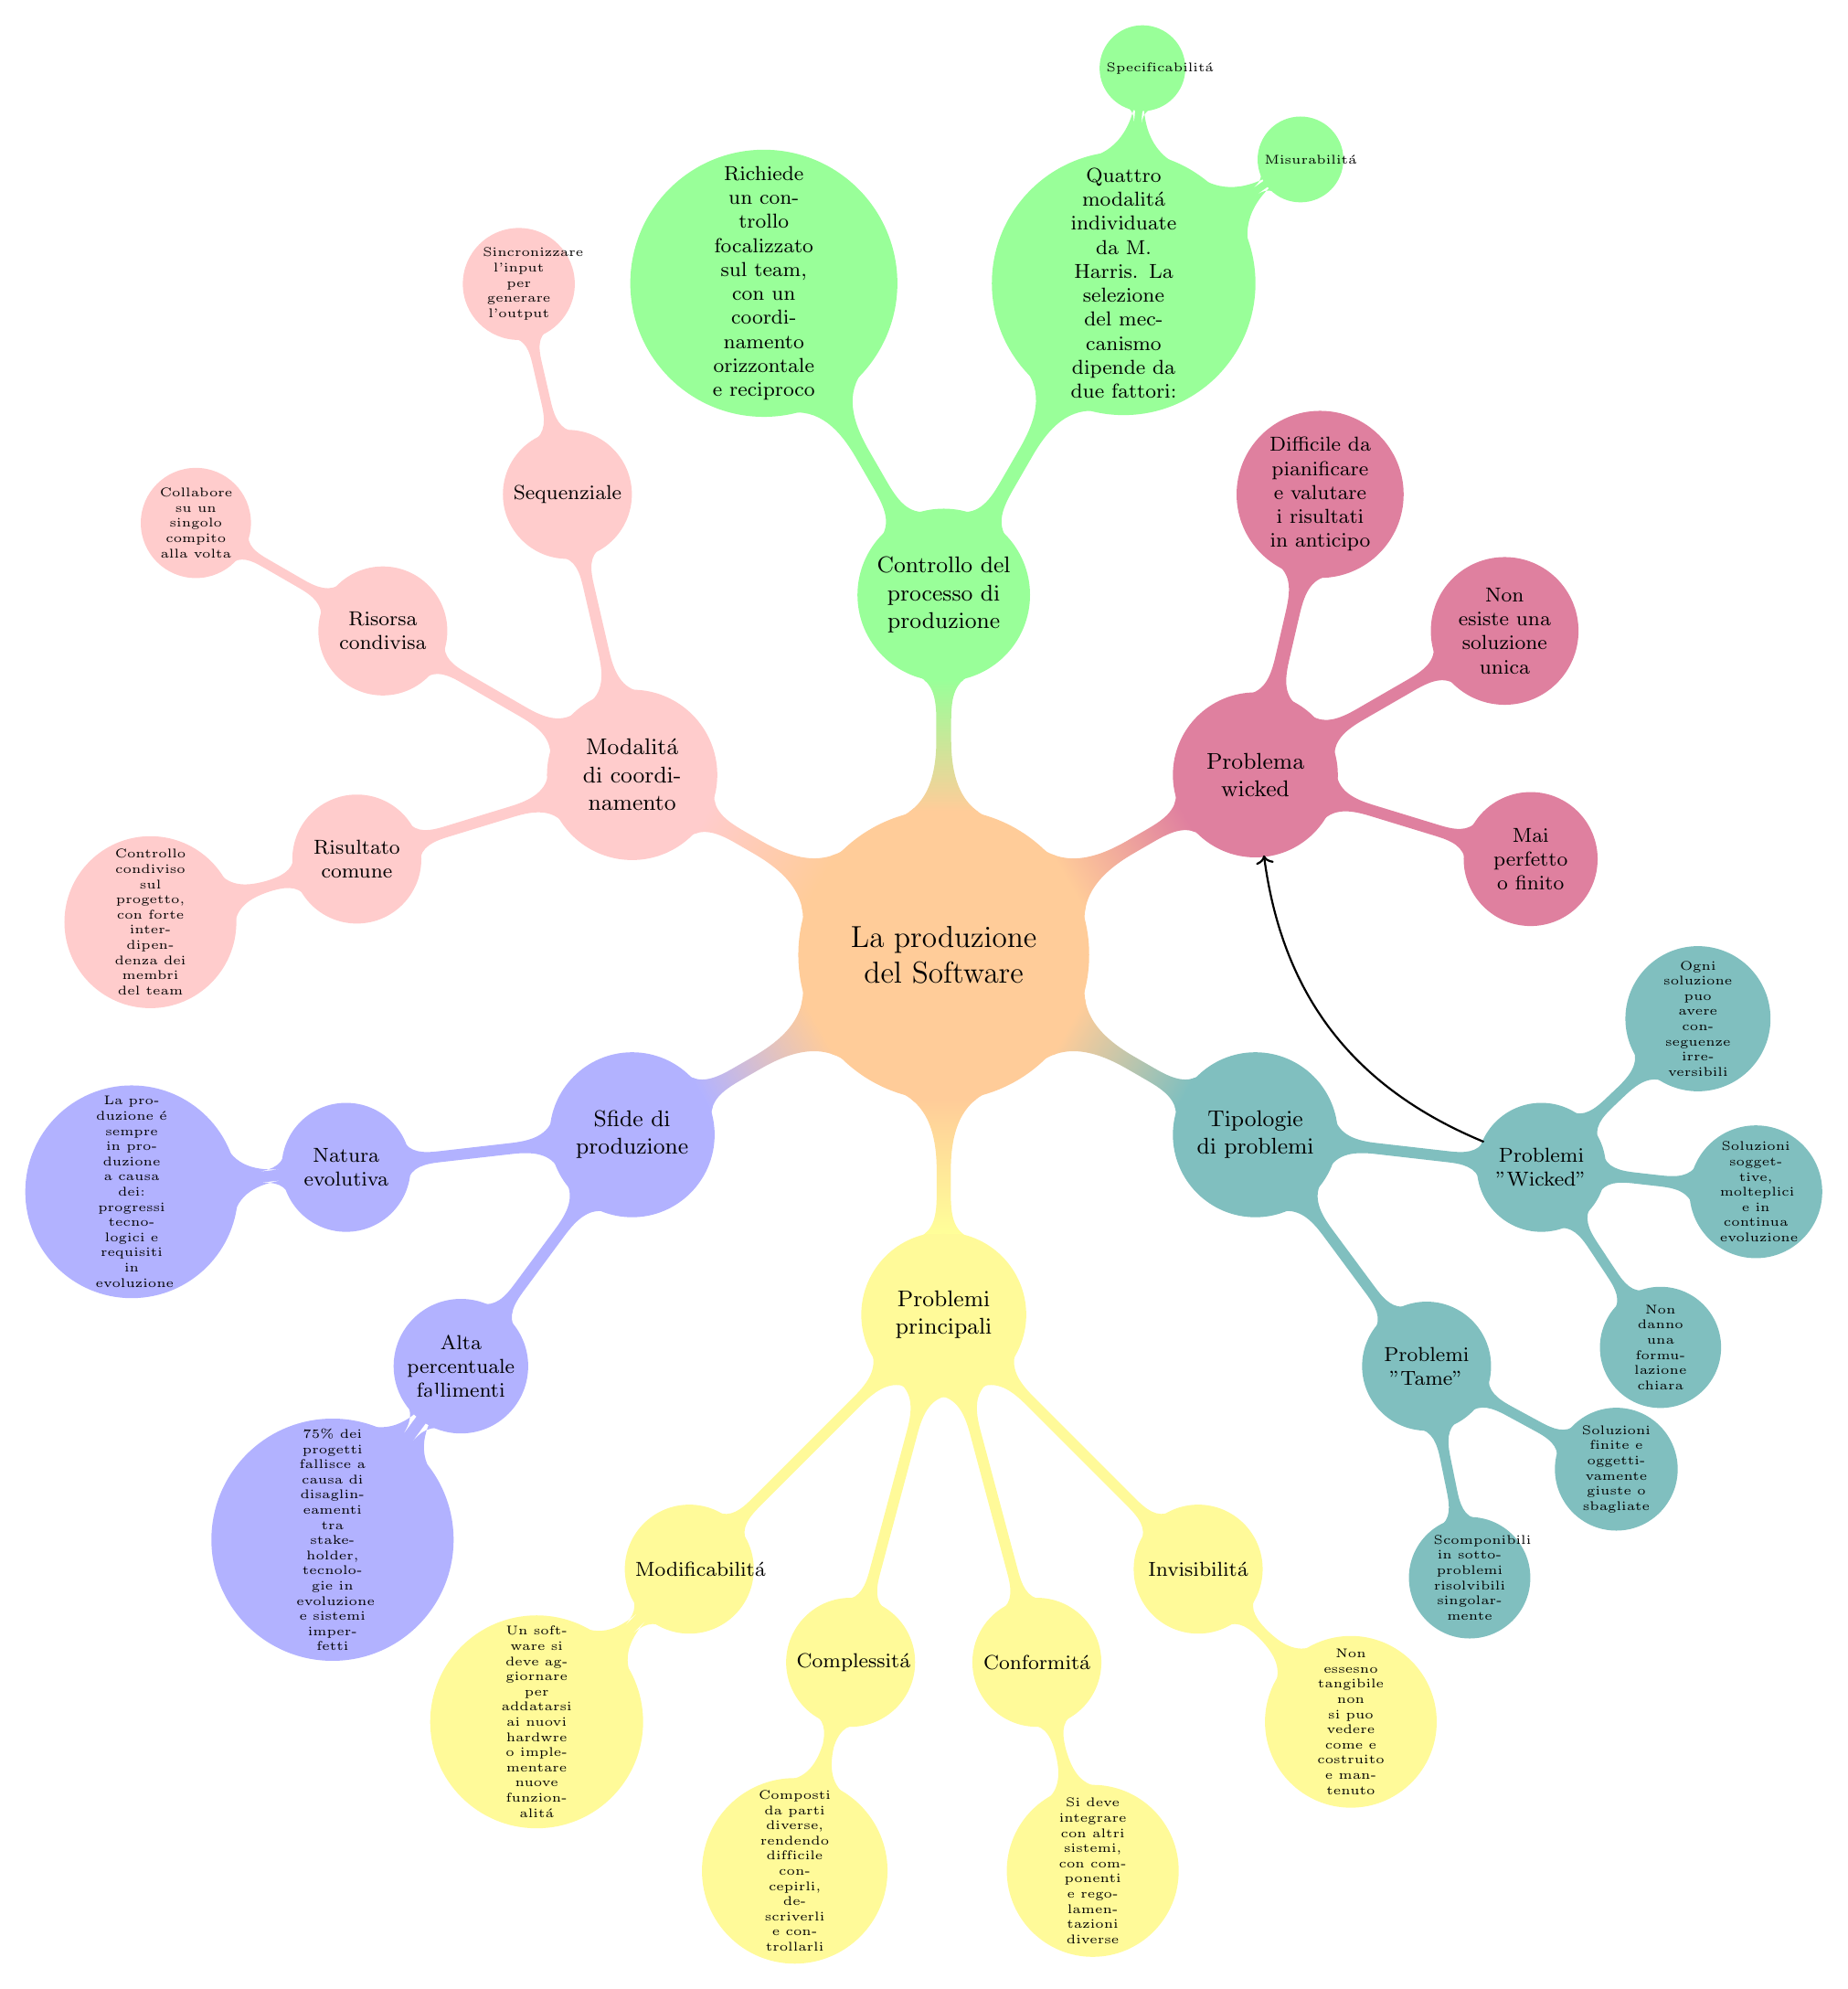
\begin{tikzpicture}[mindmap, grow cyclic, every node/.style=concept, concept color=orange!40, 
	level 1/.append style={level distance=5cm,sibling angle=60},
	level 2/.append style={level distance=4cm,sibling angle=47},
        level 3/.append style={level distance=3cm,sibling angle=50},
        level 4/.append style={level distance=3cm,sibling angle=105},]

\node{La produzione del Software}
    child[concept color=blue!30]{node{Sfide di produzione}
        child{node{Natura evolutiva}
            child{node{La produzione \'{e} sempre in produzione a causa dei: progressi tecnologici e requisiti in evoluzione}}
        }
        child{node{Alta percentuale fallimenti}
            child{node{75\% dei progetti fallisce a causa di disaglineamenti tra stakeholder, tecnologie in evoluzione e sistemi imperfetti}}
        }
    }
    child[concept color=yellow!40, level 2/.append style={sibling angle=30, level distance=5cm}]{node{Problemi principali}
        child{node{Modificabilit\'{a}}
            child{node{Un software si deve aggiornare per addatarsi ai nuovi hardwre o implementare nuove funzionalit\'{a}}}
        }
        child{node{Complessit\'{a}}
            child{node{Composti da parti diverse, rendendo difficile concepirli, descriverli e controllarli}}
        }
        child{node{Conformit\'{a}}
            child{node{Si deve integrare con altri sistemi, con componenti e regolamentazioni diverse}}
        }
        child{node{Invisibilit\'{a}}
            child{node{Non essesno tangibile non si puo vedere come e costruito e mantenuto}}
        }
    }
    child[concept color=teal!50]{node{Tipologie di problemi}
        child{node{Problemi "Tame"}
            child{node{Scomponibili in sotto-problemi risolvibili singolarmente}}
            child{node{Soluzioni finite e oggettivamente giuste o sbagliate}}
        }
        child{node[name=wicked1]{Problemi "Wicked"} %named note for arrow
            child{node{Non danno una formulazione chiara}}
            child{node{Soluzioni soggettive, molteplici e in continua evoluzione}}
            child{node{Ogni soluzione puo avere conseguenze irreversibili}}
        }
    }
    child[concept color=purple!50]{node[name=wicked2]{Problema wicked}%name for arrow
        child{node{Mai perfetto o finito}}
        child{node{Non esiste una soluzione unica}}
        child{node{Difficile da pianificare e valutare i risultati in anticipo}}
    }
    child[concept color=green!40, level 2/.append style={sibling angle=60, level distance=5cm}]{node{Controllo del processo di produzione}
        child{node{Quattro modalit\'{a} individuate da M. Harris. La selezione del meccanismo dipende da due fattori:}
            child{node{Misurabilit\'{a}}}
            child{node{Specificabilit\'{a}}}
            }
        child{node{Richiede un controllo focalizzato sul team, con un coordinamento orizzontale e reciproco}}
    }
    child[concept color=pink!80]{node{Modalit\'{a} di coordinamento}
        child{node{Sequenziale}
            child{node{Sincronizzare l'input per generare l'output}}
        }
        child{node{Risorsa condivisa}
        child{node{Collabore su un singolo compito alla volta}}
        }
        child{node{Risultato comune}
        child{node{Controllo condiviso sul progetto, con forte interdipendenza dei membri del team}}
        }
    };
\path[->, thick, black](wicked1) edge[bend left=30] (wicked2);
\end{tikzpicture}
}

%--------------- \nuova pagina ---------------
\newpage

\section{Mappa "La storia del software"} 

%--------------- Importa la mappa della storia del software --------------- 
\flushleft
\resizebox{7.2in}{!}{
    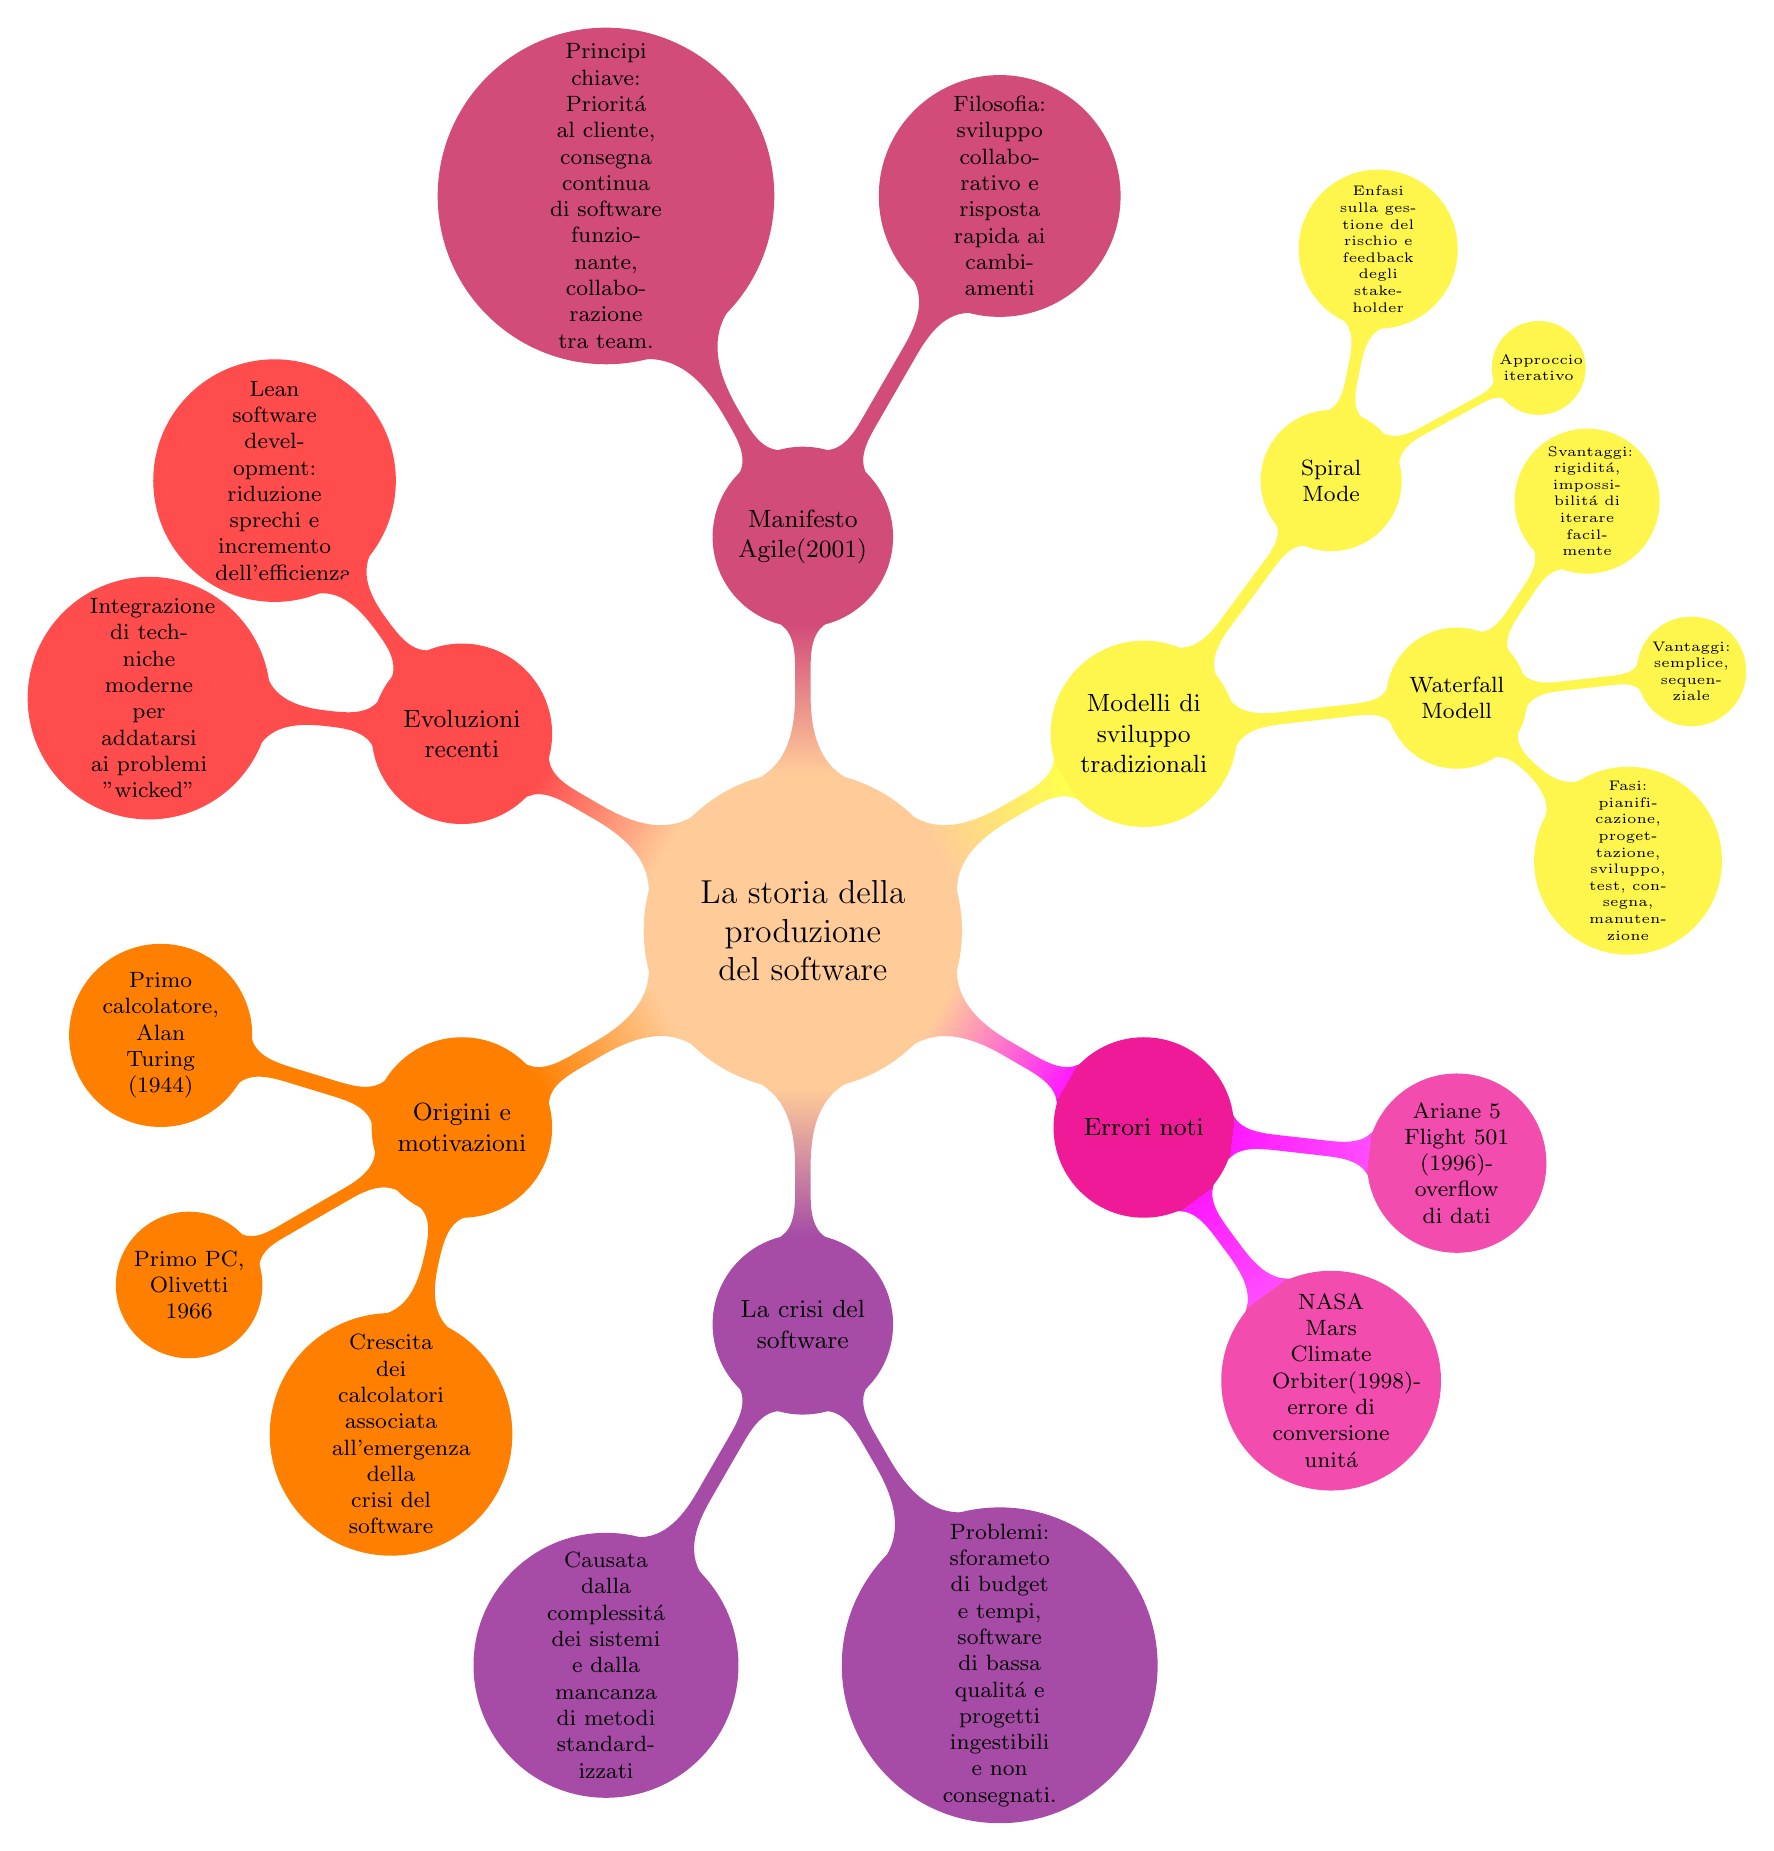
\begin{tikzpicture}[mindmap, grow cyclic, every node/.style=concept, concept color=orange!40, 
	level 1/.append style={level distance=5cm,sibling angle=60},
	level 2/.append style={level distance=4cm,sibling angle=47},
        level 3/.append style={level distance=3cm,sibling angle=50},
        level 4/.append style={level distance=3cm,sibling angle=70},]

\node{La storia della produzione del software}
    child[concept color=orange]{node{Origini e motivazioni}
        child{node{Primo calcolatore, Alan Turing (1944)}}
        child{node{Primo PC, Olivetti 1966}}
        child{node{Crescita dei calcolatori associata all'emergenza della crisi del software}}
    }
    child[concept color=violet!70, level 2/.append style={sibling angle=60, level distance=5cm}]{node{La crisi del software}
        child{node{Causata dalla complessit\'{a} dei sistemi e dalla mancanza di metodi standardizzati}}
        child{node{Problemi: sforameto di budget e tempi, software di bassa qualit\'{a} e progetti ingestibili e non consegnati.}}
    }
    child[concept color=magenta!90]{node{Errori noti}
        child[concept color=magenta!70]{node{NASA Mars Climate Orbiter(1998)- errore di conversione unit\'{a}}}
        child[concept color=magenta!70]{node{Ariane 5 Flight 501 (1996)- overflow di dati}}
    }
    child[concept color=yellow!70]{node{Modelli di sviluppo tradizionali}
        child{node{Waterfall Modell}
            child{node{Fasi: pianificazione, progettazione, sviluppo, test, consegna, manutenzione}}
            child{node{Vantaggi: semplice, sequenziale}}
            child{node{Svantaggi: rigidit\'{a}, impossibilit\'{a} di iterare facilmente}}
        }
        child{node{Spiral Mode}
            child{node{Approccio iterativo}}
            child{node{Enfasi sulla gestione del rischio e feedback degli stakeholder}}
        }
    }
    child[concept color=purple!70, level 2/.append style={sibling angle=60, level distance=5cm}]{node{Manifesto Agile(2001)}
        child{node{Filosofia: sviluppo collaborativo e risposta rapida ai cambiamenti}}
        child{node{Principi chiave: Priorit\'{a} al cliente, consegna continua di software funzionante, collaborazione tra team.}}
    }
    child[concept color=red!70]{node{Evoluzioni recenti}
        child{node{Lean software development: riduzione sprechi e incremento dell'efficienza.}}
        child{node{Integrazione di techniche moderne per addatarsi ai problemi "wicked"}}
    }
;
\end{tikzpicture}
}


%--------------- \nuova pagina ---------------
\newpage
\newgeometry{top=2cm, bottom=2cm, left=2cm, right=2cm}

\renewcommand{\bibsection}{\section*{Riferimenti}}
\addcontentsline{toc}{section}{Riferimenti}
\bibliography{data/riferimenti}

\end{document} 